\chapter{Annotation~Experiments}
\label{chap:annotation} 

In this chapter I demonstrate the practical use of the annotation tool by annotating 10 different datasets. Representative images are shown in figure~\ref{fig:datasets_all}.



\section{Datasets}

\begin{figure*}[h!]
\centering
\begin{subfigure}[t]{0.24\linewidth}
  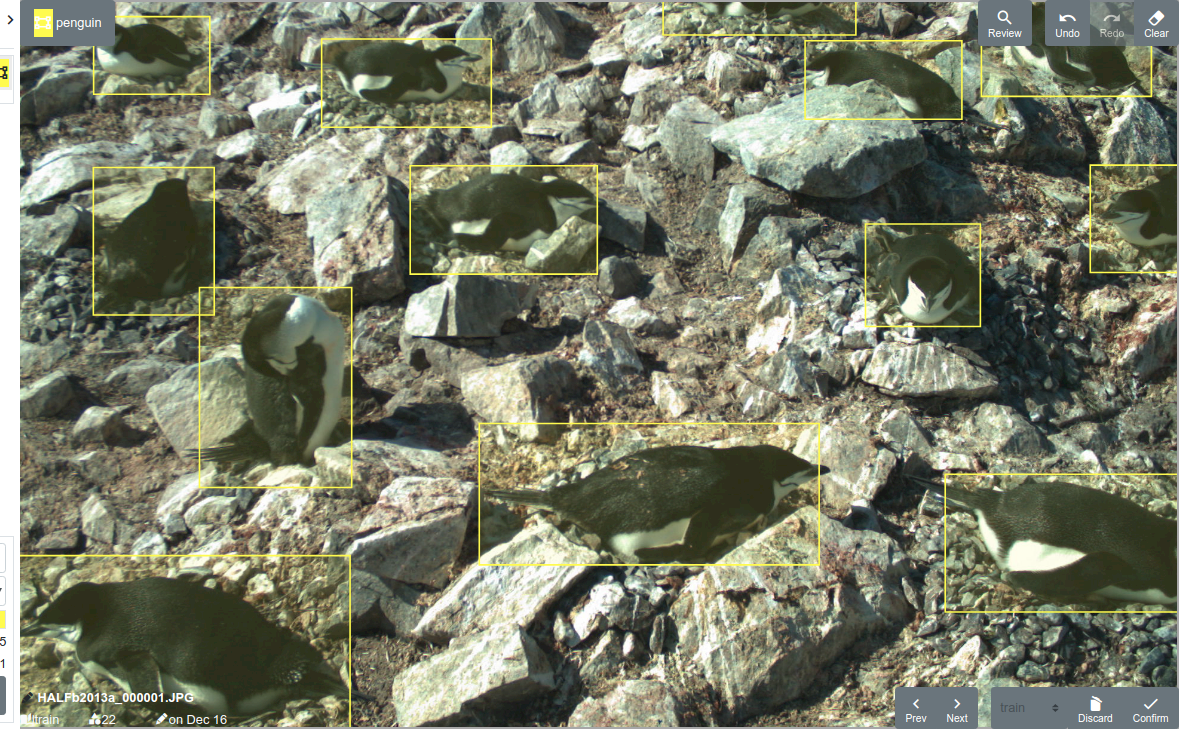
\includegraphics[width=1.0\linewidth]{figures/annotation/screenshots/penguins2.png}
   \caption{\emph{penguins}}
\end{subfigure}%
\begin{subfigure}[t]{0.24\linewidth}
  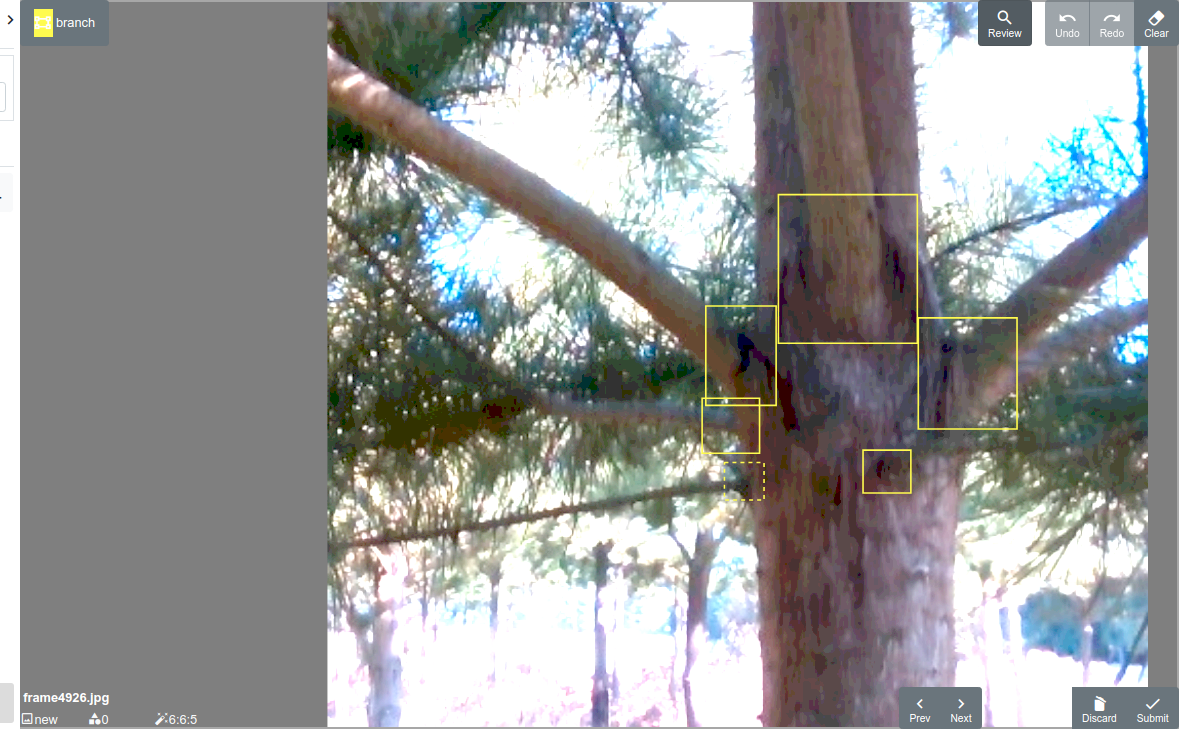
\includegraphics[width=1.0\linewidth]{figures/annotation/screenshots/branches3.png}
   \caption{\emph{branches}}
\end{subfigure}%
\begin{subfigure}[t]{0.24\linewidth}
  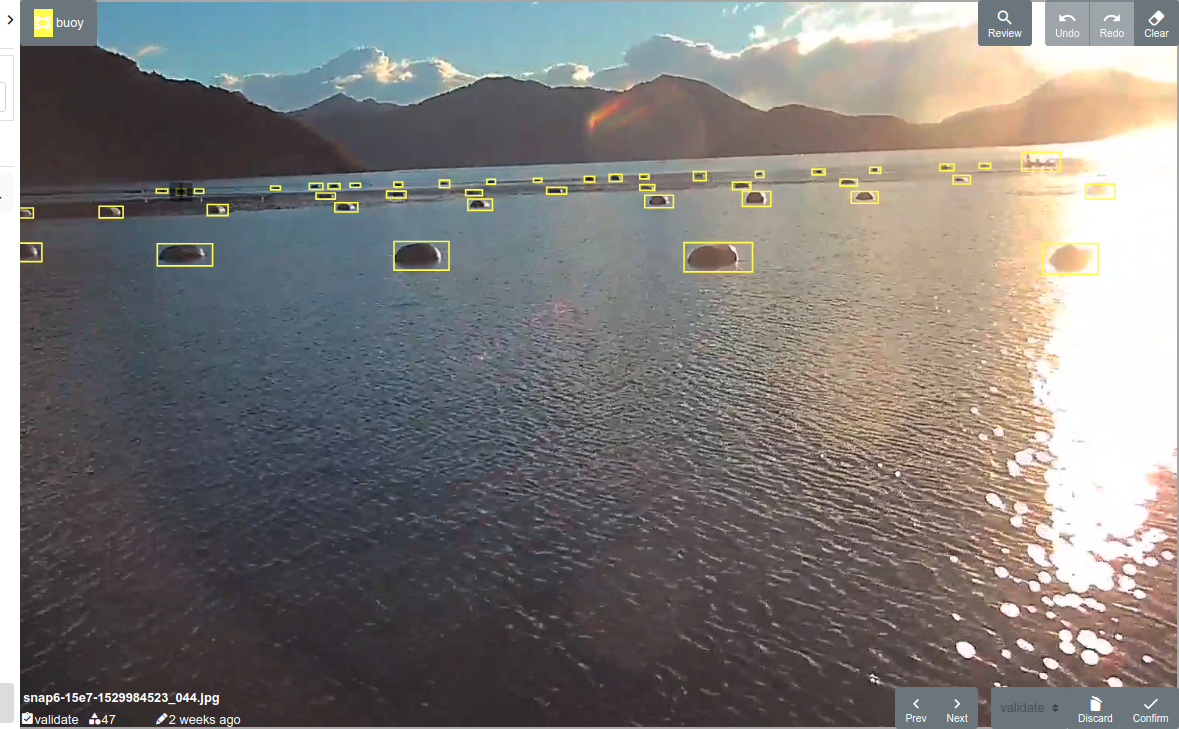
\includegraphics[width=1.0\linewidth]{figures/annotation/screenshots/buoys.png}
   \caption{\emph{buoys}}
 \end{subfigure}
\begin{subfigure}[t]{0.24\linewidth}
  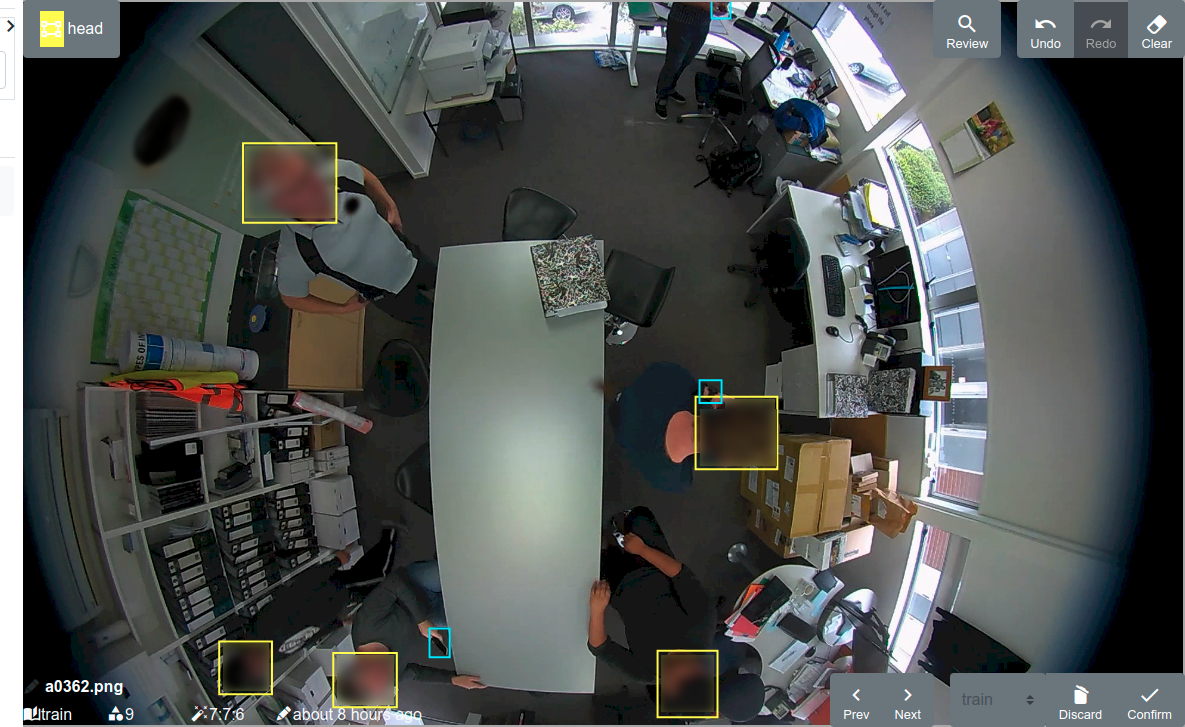
\includegraphics[width=1.0\linewidth]{figures/annotation/screenshots/victor.png}
  \caption{\emph{fisheye}}
\end{subfigure}%

\begin{subfigure}[t]{0.24\linewidth}
  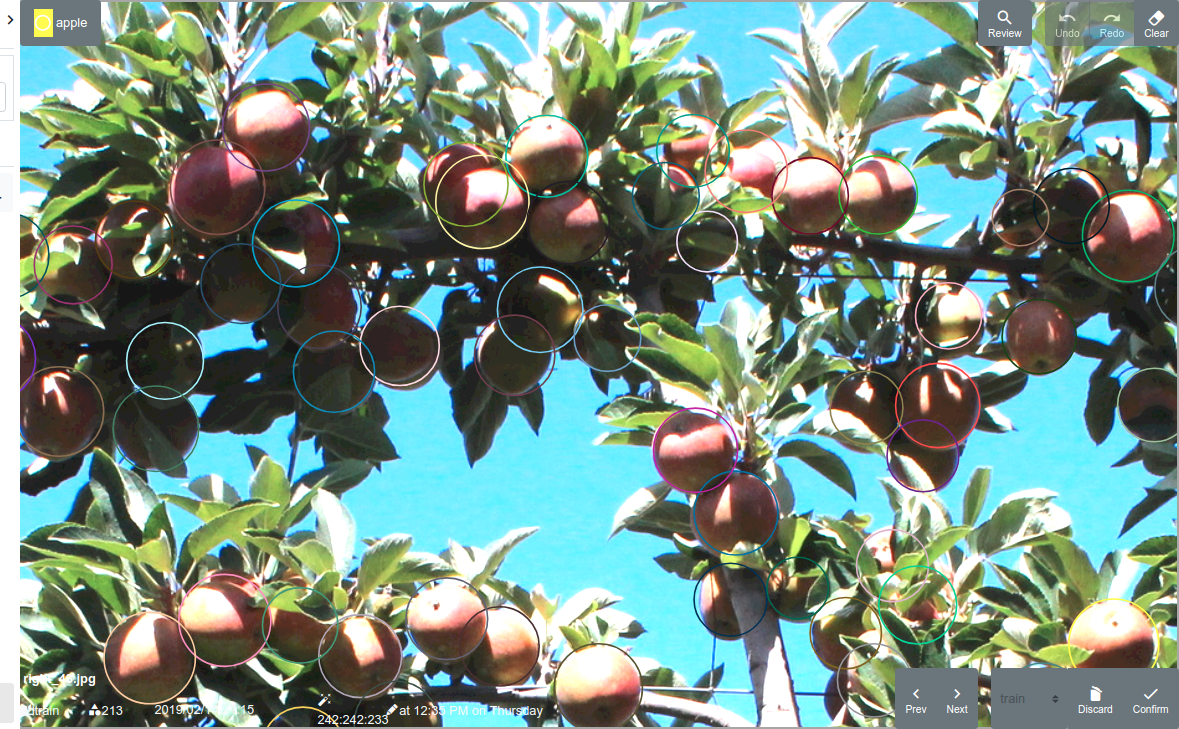
\includegraphics[width=1.0\linewidth]{figures/annotation/screenshots/apples_big2.png}
  \caption{\emph{apples}}
\end{subfigure}%
\begin{subfigure}[t]{0.24\linewidth}
  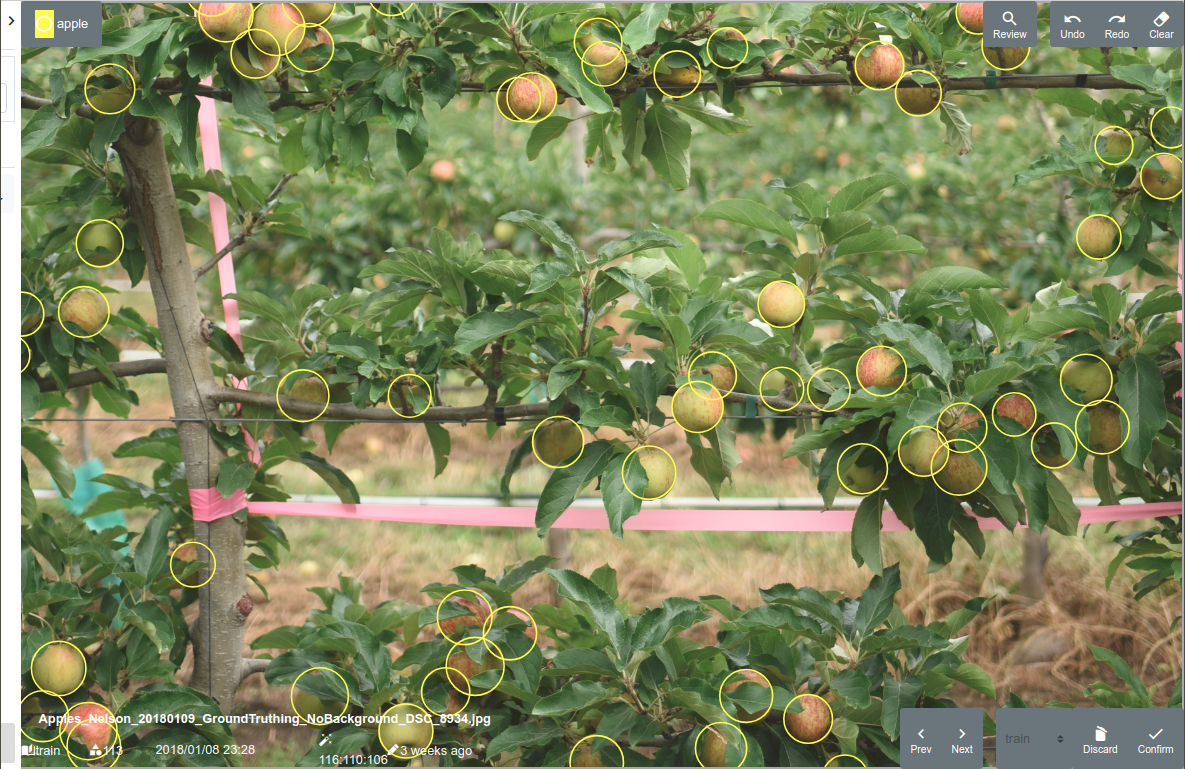
\includegraphics[width=1.0\linewidth]{figures/annotation/screenshots/apples2.png}
  \caption{\emph{apples2}}
\end{subfigure}%
 \begin{subfigure}[t]{0.24\linewidth}
  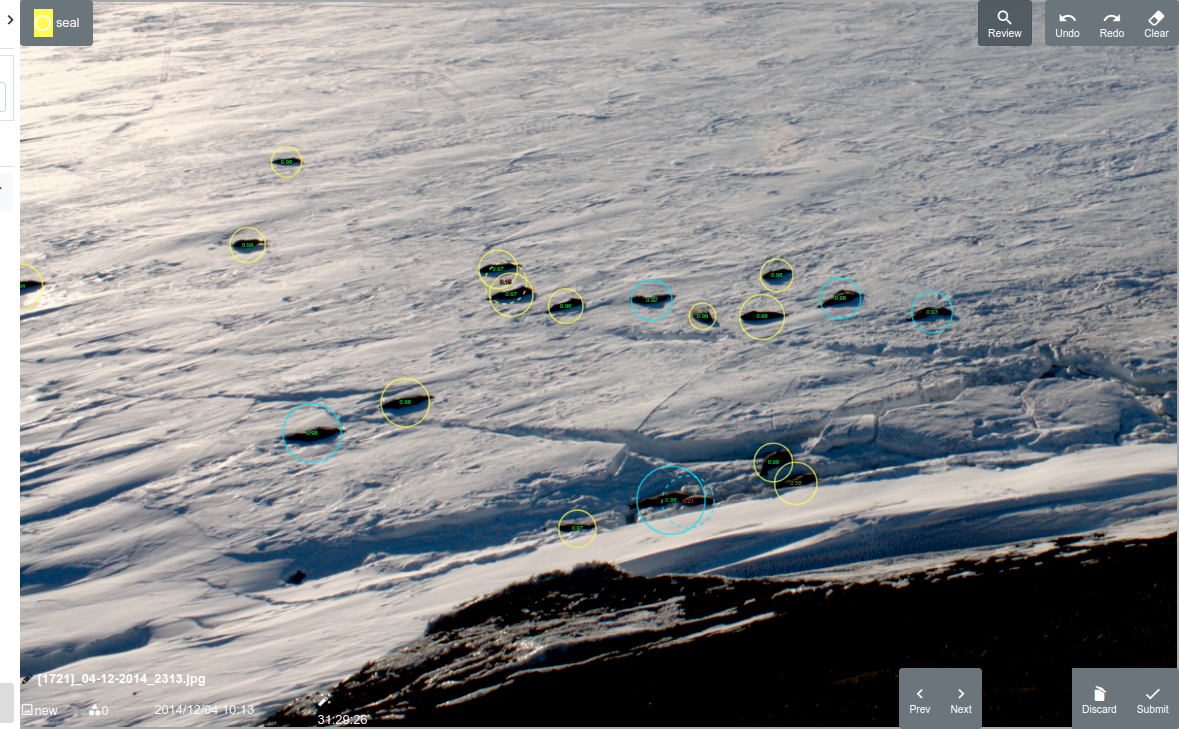
\includegraphics[width=1.0\linewidth]{figures/annotation/screenshots/seals_small2.png}
  \caption{\emph{seals}}
\end{subfigure}%
\begin{subfigure}[t]{0.24\linewidth}
  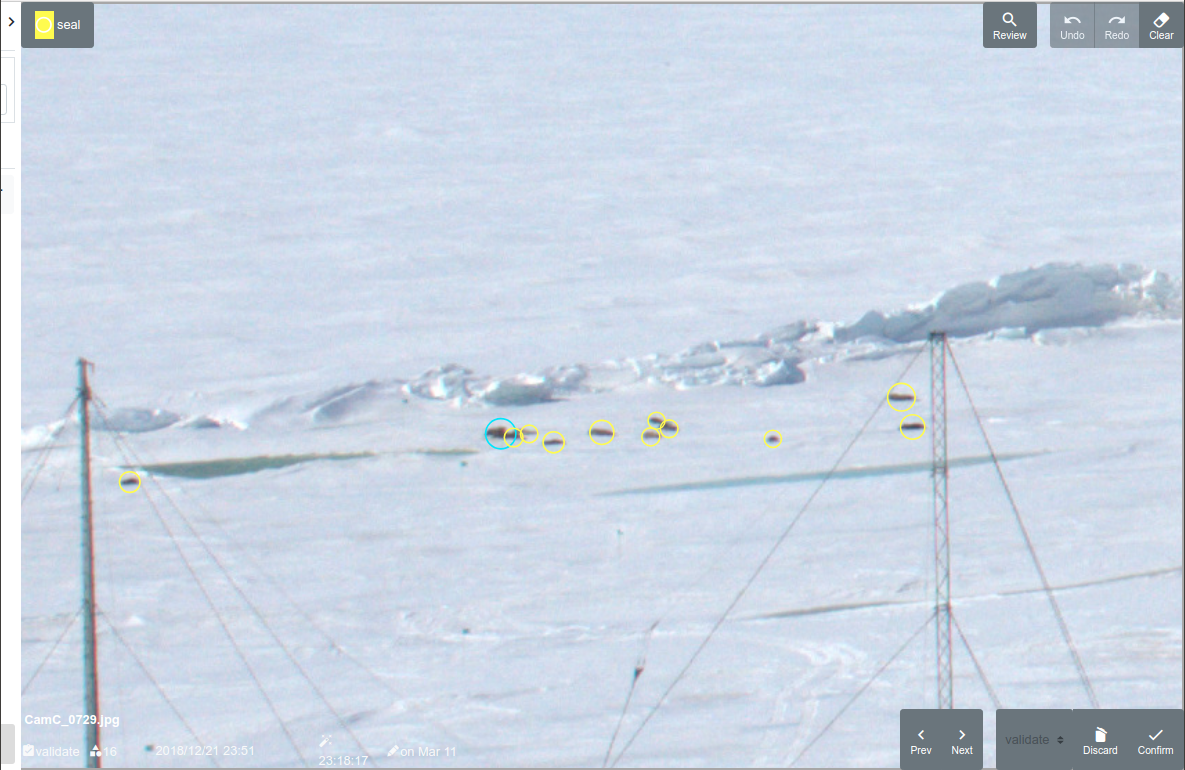
\includegraphics[width=1.0\linewidth]{figures/annotation/screenshots/scott_base_sunny.png}
  \caption{\emph{scott base}}
\end{subfigure}
\begin{subfigure}[t]{0.24\linewidth}
  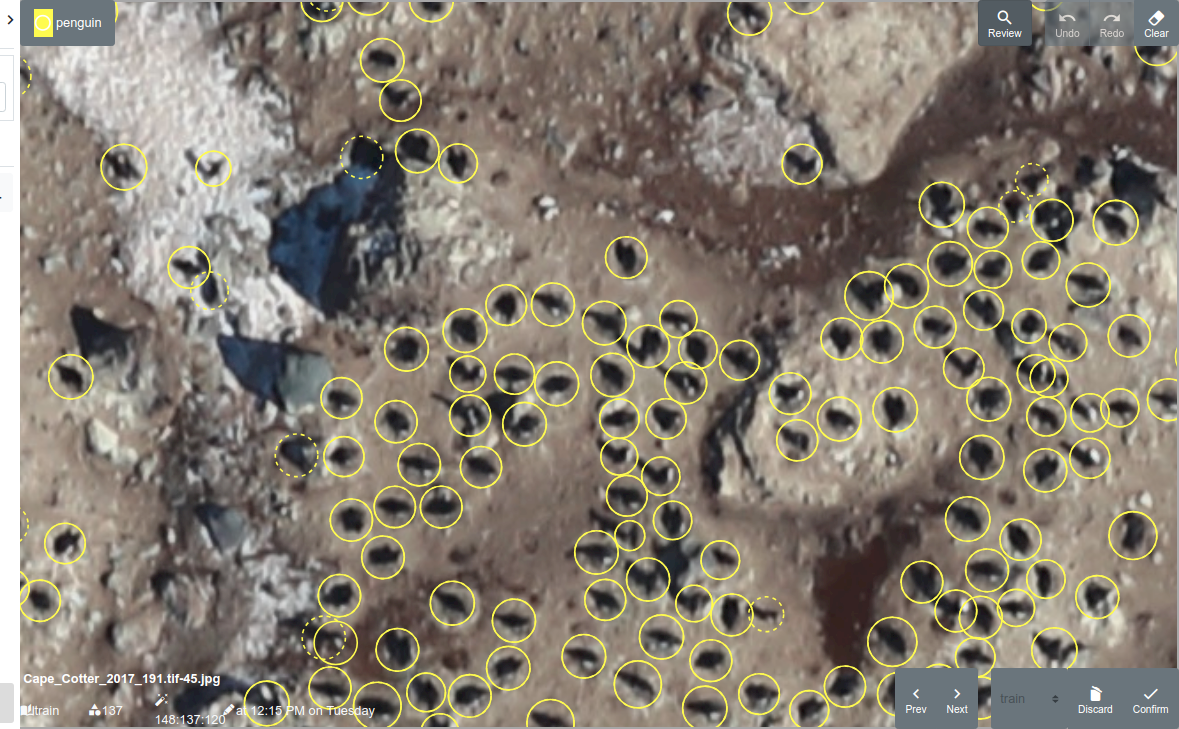
\includegraphics[width=1.0\linewidth]{figures/annotation/screenshots/penguins_aerial2.png}
  \caption{\emph{penguin survey}}
\end{subfigure}%
\begin{subfigure}[t]{0.24\linewidth}
  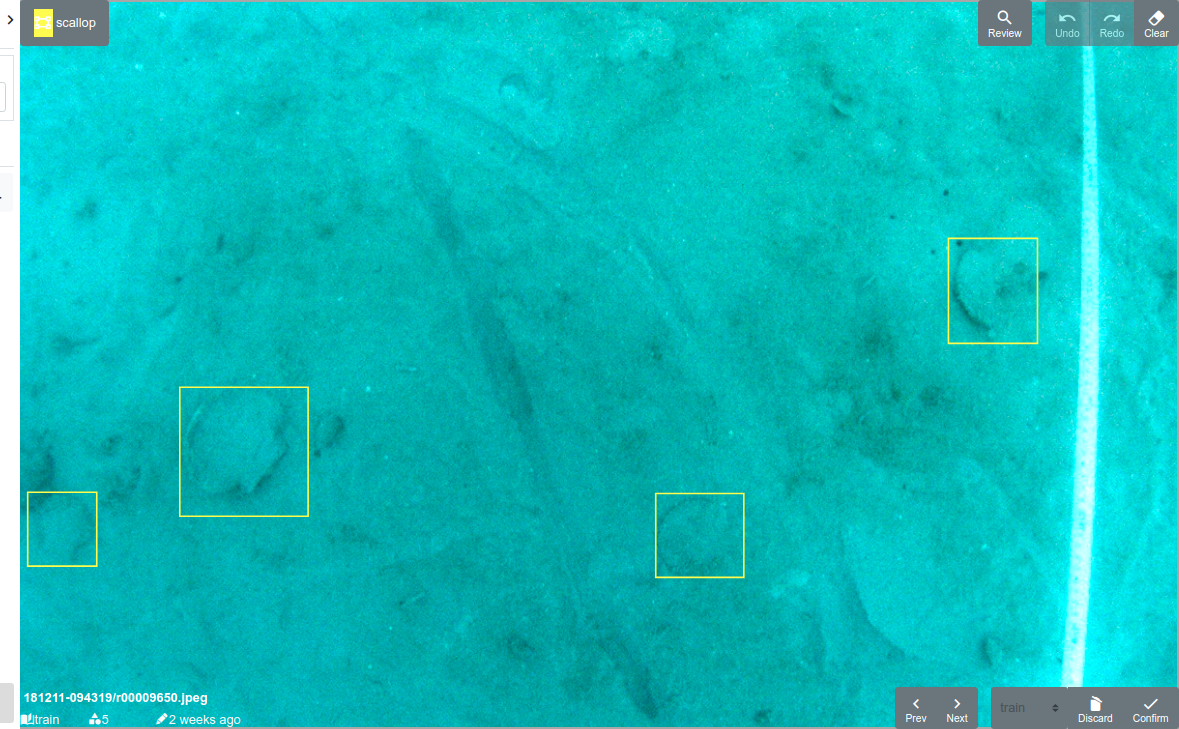
\includegraphics[width=1.0\linewidth]{figures/annotation/screenshots/scallops4.png}
  \caption{\emph{scallops}}
\end{subfigure}
\caption{Representative images of datasets (and annotations) annotated in this work}
\label{fig:datasets_all}
\end{figure*}

The datasets comprise a mix of relatively small scale image sets annotated for the sake of evaluating and developing the annotation method, image sets as test cases for future projects and a particular niche which seems suited to this kind of annotation method which is counting wildlife. In each case annotation time was between around an hour to around eight hours for the largest.

\begin{threeparttable}[!h]
\label{fig:resolutions}
\centering
\caption{All datasets, overview of number and size of annotation, number and size of image.  } 
\begin{tabular}{llllll}
dataset           & anns. & images & box length & image size                                     & val. $AP_{COCO}$ \\
\toprule
$penguins$        & 7473        & 306    & $255 \pm 118$   &  $2048\times1536$                                     & 75.9                   \\
$branches$        & 2249        & 451    & $41.5 \pm 13.9$ &  $400\times400$                                       & 62.6                   \\
$seals$           & 4351        & 240    & $68.7 \pm 20.8$ &  $3920\times1600$                                     & 80.7                   \\
$seals_b$         & 1256        & 82     & $63.4 \pm 17$   & $3920\times1600$                                                      & 72.9                   \\
$scott\:base$     & 7759        & 301    & $15 \pm 3.21$   & \shortstack[l]{$3927\times500$ -- \\ $5200\times700$}  & 81.4                   \\
$apples^1$        & 21637       & 300    & $78.4 \pm 14.9$ &  $2592\times1728$ & 51.8                   \\
$apples^2$        & 13418       & 168    & $92.8 \pm 11.9$ &  $3008\times2008$                                     & 74.5                   \\
$scallops_e$      & 3669        & 6741   & $114 \pm 40.2$  &  $1280\times1024$                                     & 65.0                   \\
$fisheye$         & 2598        & 367    & $96.6 \pm 32.7$ &  $2048\times1944$                                     & 78.9                   \\
$buoys_d$         & 7221        & 207    & $38.9 \pm 42.8$ &  $1920\times1080$                                     & 42.7                   \\
$penguin\:survey$ & 13210       & 352    & $22.6 \pm 2.11$ & \shortstack[l] {$406\times405$ -- \\ $672\times448$}     & 61.6               \\
\bottomrule
\end{tabular}
\begin{tablenotes}
\small
\item $*$ Subscripts denote different annotator, for example $seals_b$ is annotated by annotator $b$ where images from the same distribution of images (not necessarily the same images) are annotated by different users.  
\item $\ddagger$ Superscript denotes images from a different distribution of images
\item Datasets specified without subscript are annotated by the author.
\item $\dagger$ A bug relating to anchor box positioning impacted object detection. 
\end{tablenotes}
\end{threeparttable}


\begin{itemize}
    \item{\bf{penguins}}\par
A dataset used in the development of the annotation tool, primarily because the object detector performed well on the images after only a few annotated images and the relative uniformity of the images. The images used are a subset 'HALFb'  of the \emph{penguin dataset} \cite{PenguinData} used for counting using point annotations \cite{Arteta2016}. 
    \item{\bf{branches}}
A dataset annotated as a test run for cut-point detection, where branch intersections (including hidden ones) are annotated with boxes by including the collar of the branch and a piece of the branch. Images are randomly sampled from a large set of frames extracted from several video sequences of orbits around trees. Images are lower resolution than other image sets $ 400\times400 $ images, and a number of images have poor contrast.

    \item{\bf{buoys}}
A trial run for the monitoring mussel buoys, the idea is to monitor the growth of mussels by visually examining the height of the buoy out of the water; out of the scope of this work. Object detection is used as a first step however and used to determine a water plane. Images are sampled from video sequences taken from a camera fixed to another mussel buoy. As a result the view angles are somewhat limited, but do change as the buoy rotates with the swell, weather and lighting conditions give a variation in appearance. 

Although image resolution is reasonably high $1920\times1080$, there are considerable visible artefacts from video compression. Buoys in the distance become very tiny, and were ignored once they became hard to distinguish. Buoys also tended to line up and occlude each other, these buoys were also ignored.


    \item{\bf{fisheye}}
    
A test for detecting people (heads) and cellphones in roof mounted fisheye camera images. Trained models for human detection (and pose recognition) are readily available but fail on fisheye images because the orientation and scale of an object changes dependent on position in the image. Person detection worked almost immediately after a handful of images with only minor corrections required, cellphone detection required more intervention, but began to work reliably towards the end of annotation. Experiments afterwards showed that the high resolution $2048\times1944$ was necessary to detect the cellphones; detection failed at half resolution.

    \item{$\mathbf{apples^1}$}

A set of images of trellised apple trees with many apples per image, only apples in the foreground were annotated, small apples and cherries in the background provided distraction. Leaves occluded a large number of apples, however all apples which could be approximately localised were annotated. Often it is possible to guess quite accurately at the location of the apple because a section of the curved outline can be seen, though harder to accurately guess the size. 

Images were taken with a high resolution DSLR camera and scaled to half resolution $2592\times1728$; apples in the photos at this resolution are large (from 50 to 200 pixels, median around 80). Despite only annotating 300 images, this dataset has the most annotations at over $22000$. Lighting was often less than ideal with direct sunlight causing poor contrast in many images.
    
    \item{$\mathbf{apples^2}$}
    
Another set of images of trellised apple trees, compared to \emph{$apples^1$} having a higher degree of  photographic consistency (resulting in more consistent sizes and number of apples), better focus on the foreground (less distracting background, some images additionally given a black backdrop). These differences manifest themselves in  in the difference in validation accuracy seen in figure~\ref{fig:validation}, reaching a higher accuracy than \emph{$apples^1$}.

Of a similar resolution to \emph{$apples^1$}, some images captured as portrait where all images in \emph{$apples^1$} are landscape. The same annotation strategy was used between both sets, annotate all apples which can be localised.

    \item{\bf{seals}}
Time series images (10 minutes apart) taken of a part Antarctic Weddell seal colony around Turtle Rock, an island around 12km north of Scott Base, for a three week period from the 28th November to 19th of December 2014. The purpose for this monitoring is to establish haul out patterns where seals sit on the ice (in order to avoid predation).  

Images were taken from a high resolution DSLR camera and cropped to give a resolution of $3920\times1600$. The images were annotated twice (different images in both cases), and separate test sets (the same images in both cases) were annotated created before annotation began. From a set of $3000$ images, in the first case $240$ images were annotated by the author and the second $82$ by user $b$, the test set comprises of $46$ images.

The seals generally sat well separated and very clearly distinct, except for mother and pup which often sat right next to each other. Lighting was occasionally quite difficult. Seals were annotated as two classes, either: (a) single seal (b) mother next to pup.  The misclassification of mother and pup vs. single seal was the largest source of error during annotation and in validation. Often disambiguating the two is difficult for a human without viewing images in the time series, where it becomes apparent due to motion.

More details can be found in section~\ref{sec:case_seals}.

    \item{\bf{scott base}}
Again time series images (10 minutes apart) taken of Weddell seals around Scott Base, Antarctica. Two different views were used in this work (three were captured, but in the time period used here the third contained few seals). The purpose is for population monitoring between years when Scott Base is renovated in the coming years, to evaluate the impact on seal population.

Two different DSLR cameras were used each with a different viewpoint (and different image size). Images were cropped to the regions containing seals, as such were very wide, $5000\times700$ from one viewpoint. The viewpoints unlike the \emph{seals} images were from far away and the seals were tiny (a mean of $15$ pixels diameter) with considerable blurriness.  
    
More details can be found in section~\ref{sec:case_seals}.
    
    \item{\bf{penguin survey}}
The images are from the Adélie Penguin Census \cite{Lyver2014}, an aerial photographic survey (taking place from 1981 until present) in which a complete census of the Adélie penguin population is taken by counting nesting pairs. High resolution photographs are taken from from 2000-2500 feet.

Three separate annotations are performed; two of them from images comprising part of two large colonies, one a complete smaller colony in 3 separate images. In each case the large images are broken into small images for practical reasons. In terms of the number of annotations the software can handle, as well as the number of annotations which is practical for an annotator to check in one go.
    
The images once chopped into pieces are relatively small, but still contain large numbers of penguins, comparable to $apples^2$ in terms of annotation per image (see figure~\ref{fig:instances_image_plot}). The penguins themselves are small and blurry, with two forms, either sitting or standing which are easily confused, and also easily confused (and considerably ambiguous) with the shadows in rocky areas.  
    \item{\bf{scallops}}
    
The images are drawn from video frames taken by an underwater \gls{ROV} used to survey a small seabed area containing scallops. The images are unique from others used in this work in that the object instances are very sparse; there are many images with no scallop. 

The images are part of a project intending to survey scallops, and eventually develop methods of mechanically harvesting scallops. The usual method of harvesting scallops is by dredging the sea floor, an environmentally destructive method. By harvesting scallops individually the destruction of the sea floor can be avoided.

These images are an initial test run of both image capturing and annotation. The lighting on the \gls{ROV} went out mid capture, leading to approximately half the images appearing in good lighting and the other half in dim blue natural light. The point of view changed mid capture, some images are forward facing, others downward facing. The images also often traversed backwards and forwards across the same areas, thus limited visual appearance (often seeing the same scallop repeatedly). 

\end{itemize}


\begin{table}[]
\centering
\caption{ Annotation statistics and user actions for each dataset }
\label{fig:annotation_table}
\begin{tabular}{llllll}
dataset           & actions & anns. & \shortstack {ann. time \\ (minutes)} & \shortstack{instances \\ per minute} & \shortstack{actions \\ per ann.} \\
\toprule
$penguins$        & 2,070   & 7473        & 140                       & 53.5                 & 0.28                   \\
$branches$        & 745     & 2249        & 63                        & 35.7                 & 0.33                   \\
$seals$           & 587     & 4351        & 89.8                      & 48.5                 & 0.13                   \\
$seals_b$         & 453     & 1256        & 76.4                      & 16.4                 & 0.36                   \\
$scott\:base$     & 1,499   & 7759        & 123                       & 63.1                 & 0.19                   \\
$apples^1$        & 5,542   & 21637       & 511                       & 42.4                 & 0.26                   \\
$apples^2$        & 3,710   & 13418       & 364                       & 36.9                 & 0.28                   \\
$scallops_e$      & 2,065   & 3669        & 561                       & 6.54                 & 0.56                   \\
$fisheye$         & 337     & 2598        & 58.4                      & 44.5                 & 0.13                   \\
$buoys_d$         & 1,230   & 7221        & 234                       & 30.9                 & 0.17                   \\
$penguin\:survey$ & 1,616   & 13210       & 120                       & 110                  & 0.12                  \\
\bottomrule
\end{tabular}
\end{table}



\section {Evaluation methods}
\label{sec:ann_evaluation}

The primary method of evaluation used in this work is that of \emph{continuous testing} whereby it is possible to characterise how the annotation process changes over time; how the model's predictions impact on the actions taken by the annotator, the type of actions and time required, and the accuracy of the model's predictions.

User edits are logged, along with predictions provided by the model (the starting point for annotating each image), and the final set of annotations submitted by the user. The accuracy of detections are verified directly by the user, giving both continuous testing of the model predictions as well as providing useful feedback to the user of the system. 

The types of actions as well as the timing can provide useful cues as to the difficulty of the task, and the level of assistance provided by the object detection model. 

I break down these actions, and the relation of the actions to the original set of detections and the performance of the object detector in a few different ways: categorise the action types and frequencies, categorise the corrections applied to each annotation, and lastly use a locally weighted \gls{AP} to quantify object detection performance on newly annotated images.

\subsection{User actions}

The various user actions are discussed in section~\ref{sec:user_interface} more detail. For the purposes of this chapter the user actions are broken down into categories:

\begin{itemize}
    \item {\bf transform}: an annotation is transformed (scaling, translation, corner dragged).
    \item {\bf confirm}: a weak detection is confirmed. This may also includes a transformation of bounding box, but as it is performed as one action.
    \item {\bf delete}: one or more annotations are deleted.
    \item {\bf add}: a new annotation is added.
    \item {\bf set class}: the class of an annotation is changed.    
    \item {\bf submit}: an image is submitted.    
\end{itemize}

\subsection{Annotation corrections}
\label{sec:corrections}

Another way of analysing the annotation process is to categorise each annotation by the nature of corrections applied to it (or used to create it) from predictions of the object detector. This differs from just looking at user actions because: (a) multiple actions may be performed on one annotation, for example, a scaling and a translation, or changing the class and translation (b) one action may modify multiple annotations, frequently a deletion of multiple false positives at once.

The following definitions are used:

\begin{itemize}
    \item {\bf positive}: a high confidence detection unchanged after verification.
    \item {\bf modified}: high confidence detection where either the box annotation or the class label has been modified.
    \item {\bf weak positive}: a weak detection confirmed translated).    
    \item {\bf false negative}: an object which was missed by the object detector and annotated manually by the user.    
    \item {\bf false positive}: an incorrect high confidence detection deleted by the user.
\end{itemize}

\subsection{Measuring progress with Cumulative Annotation Time}
\label{sec:ann_time}

\begin{figure}
\centering
  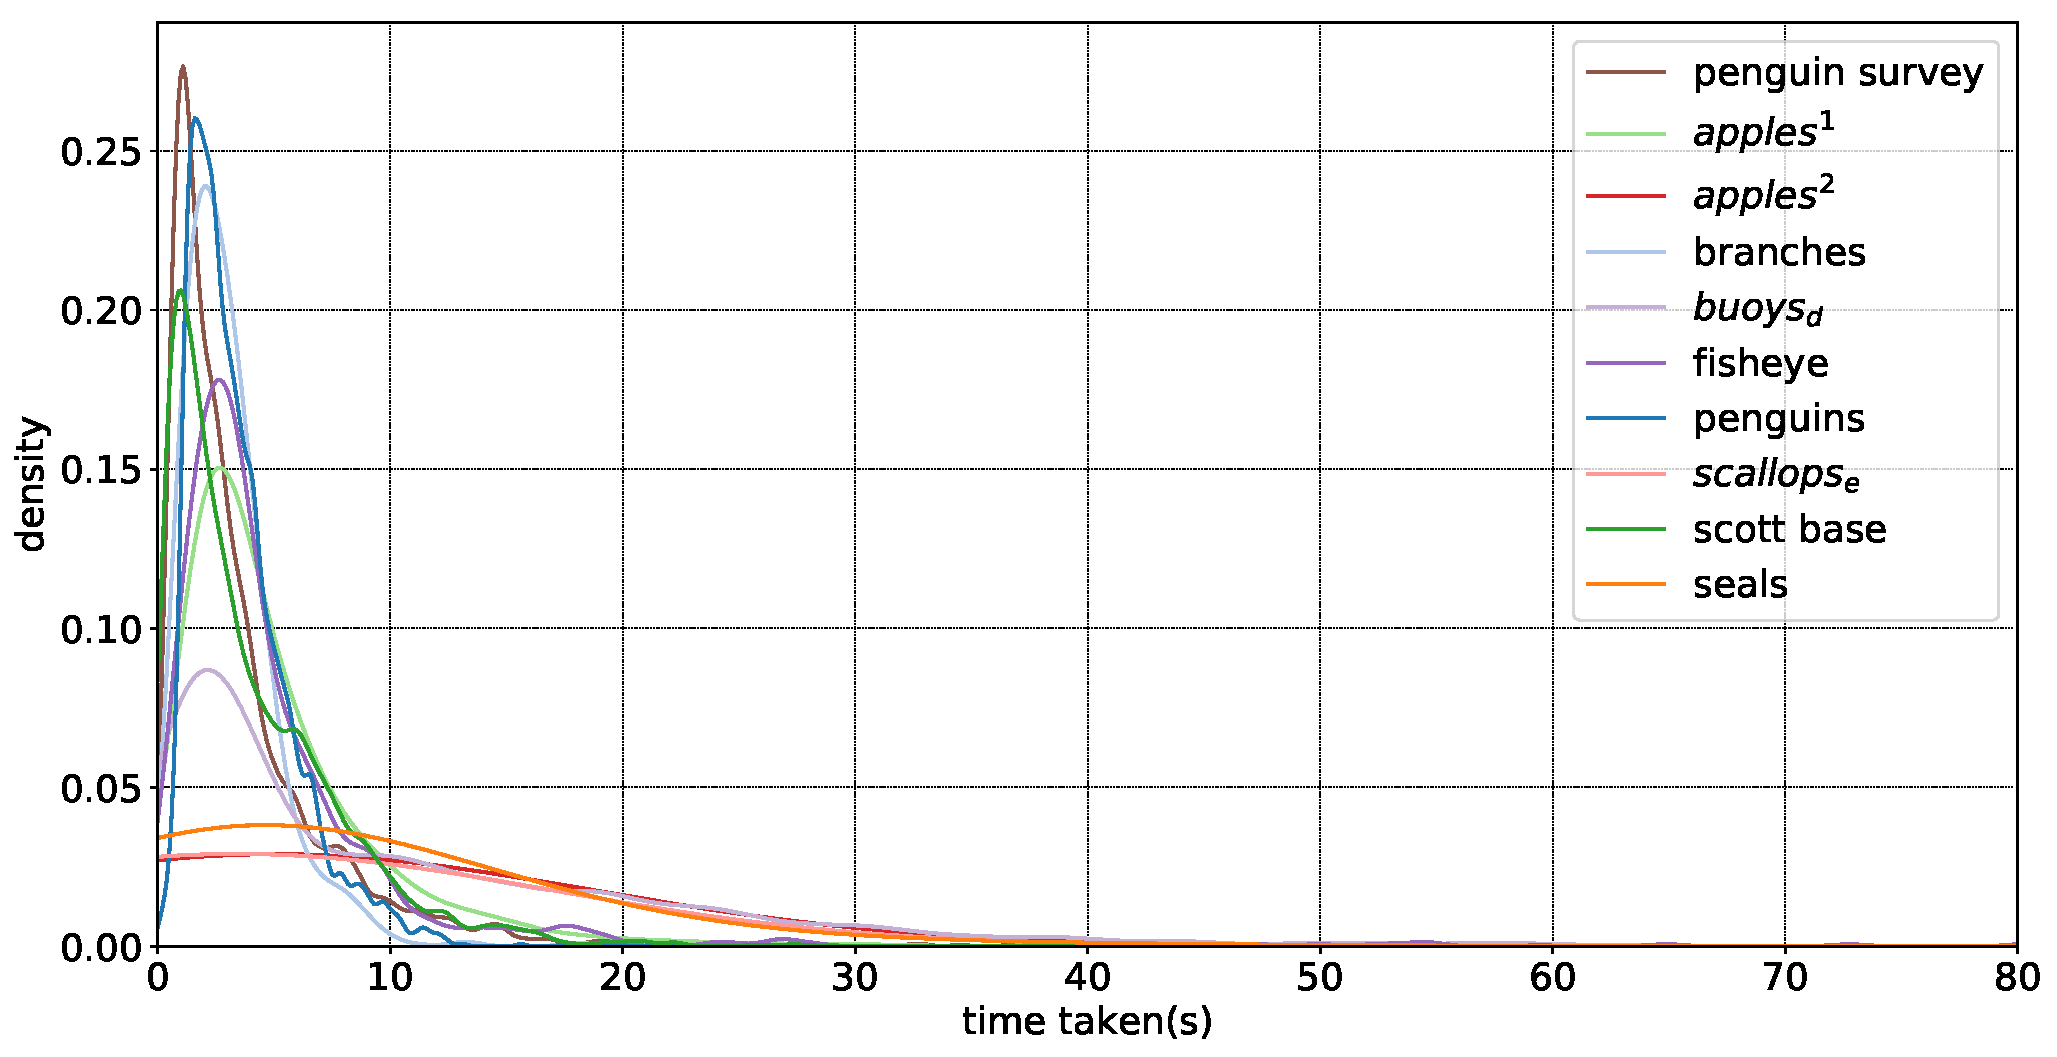
\includegraphics[width=1.0\linewidth]{charts/summaries/time_density.pdf}
  \caption{Time per action distributions for different dataset annotation}
  \label{fig:annotation_time_density}
\end{figure}

Measuring progress over the period of annotating a dataset. Due to the variation between images, the granularity of recorded annotations (often several hundred per image) the raw actions need to be grouped (for example, histograms over time). There are several ways progress could be measured in terms of annotation progress, such as the time spent since annotation began, the number of images or annotations submitted or the focus of this chapter, \gls{CAT} the total time the user spend has spent actively using the tool.

In section~\ref{sec:schedule}, trials incrementally enlarging the dataset showed the accuracy in validation to be strongly correlated to the number of examples used. For this reason we decide to use annotation progress (as opposed to training time for example) to visualise progress.

\subsection {Break detection}
\label{sec:break_detection}

The annotation logs recorded in this chapter were not taken in a controlled experimental setting, although an effort was taken to be consistent in datasets annotated by the author. Datasets annotated by others' can be seen to have more variability. It was therefore necessary to detect breaks where annotation was paused mid-image. Any action was capped at a maximum one minute for this purpose. Ideally this would have been detected directly in the tool by detecting lack of input or loss of focus, and future studies will take this approach. 

Figure~\ref{fig:annotation_time_density} shows the distribution of times per action for different annotation efforts where any action taking more than a minute is a significant outlier in most cases. An obvious discrepancy can be seen between the \emph{scott base}, \emph{seals} and \emph{scallops} datasets, this is because the video sequences are useful in resolving ambiguity and more time is spent looking forward and backward at previous frames.

\subsection{Visualisation}
\label{sec:visualisation}

In order to visualise trends in the user action types a fixed size density estimation is used with gaussian kernel, $\sigma=5 minutes$. This approach is taken for both user actions, annotation correction types, the rate of annotations and using a weighted \gls{AP} to quantify overall detector performance at a particular point in  time.

Annotation actions, corrected annotation types are all deemed to occur at the \gls{CAT} the image is submitted. Even though actions occurred at distinct points during an image annotation, the interest is in overall trends rather than particular trends within annotating each image. 

\subsection {Locally weighted Average Precision}
\label{sec:noisy_trends}

To give a single metric for object detection performance where parts of a dataset are more important than others I use a weighted \gls{AP}. The object detector's predictions are compared against the users final annotations. A standard matching procedure is performed for all images (as opposed to tracking the user edits as in section~\ref{sec:corrections}).

In order to align with user actions across \gls{CAT}, a locally weighted \gls{AP} is used. To evaluate the locally weighted \gls{AP} at a particular point in cumulative annotation time, each image is given a weight according to it's time difference from the image \gls{CAT}. As above the gaussian kernel with $\sigma=5 minutes$ is used.

Annotations in each image are weighted by the image weight for the purposes of counting false positive, false negative and true positive counts. From there weighted precision and recall and \gls{AP} are computed exactly as normal. See section~\ref{sec:evaluation_metrics}.


\section {Dataset overview}
\subsection {Size distribution}

\begin{figure}[ht]
\centering
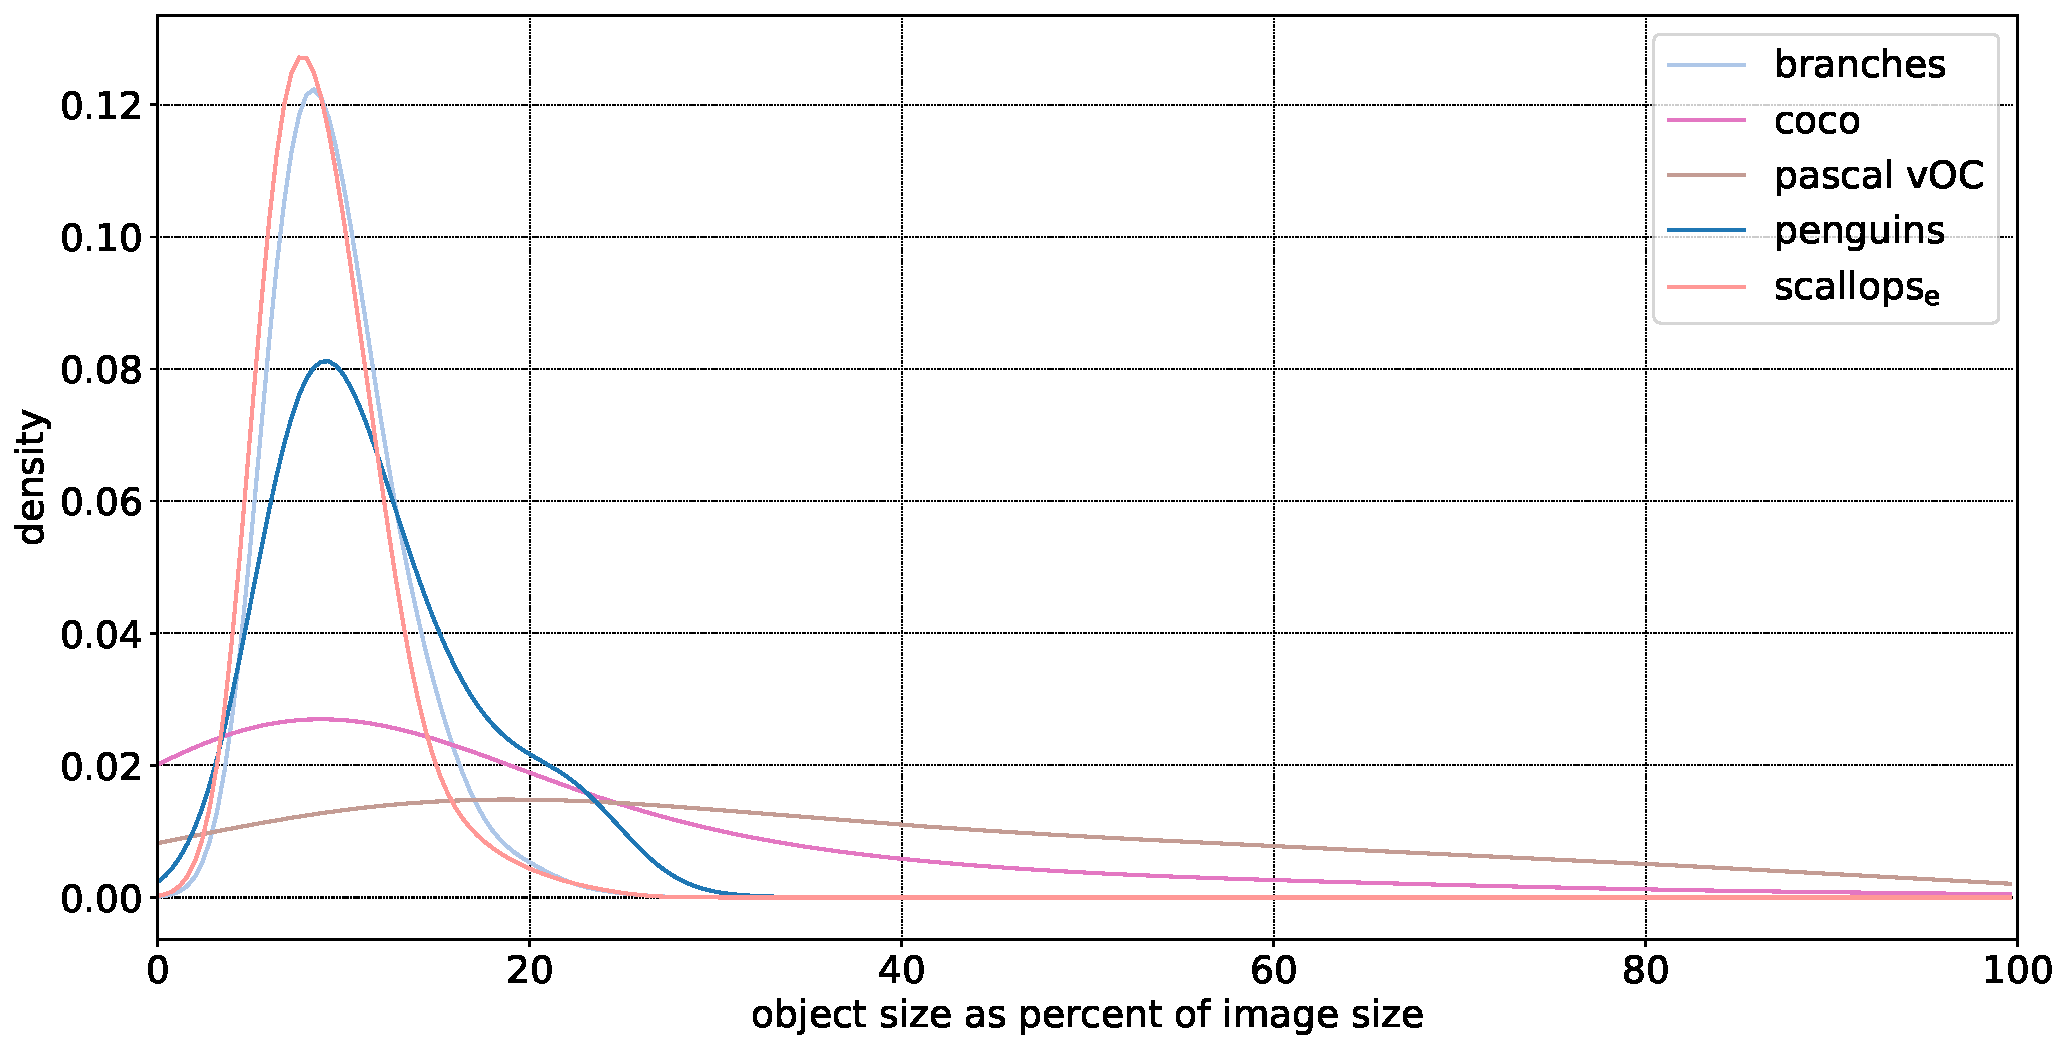
\includegraphics[width=1.0\linewidth]{charts/summaries/sizes_density.pdf}
\caption{Object bounding box size distributions as percent object to image size (average of width and height ratios) }
\label{fig:box_sizes}
\end{figure}
 

\begin{figure}[ht]
\centering
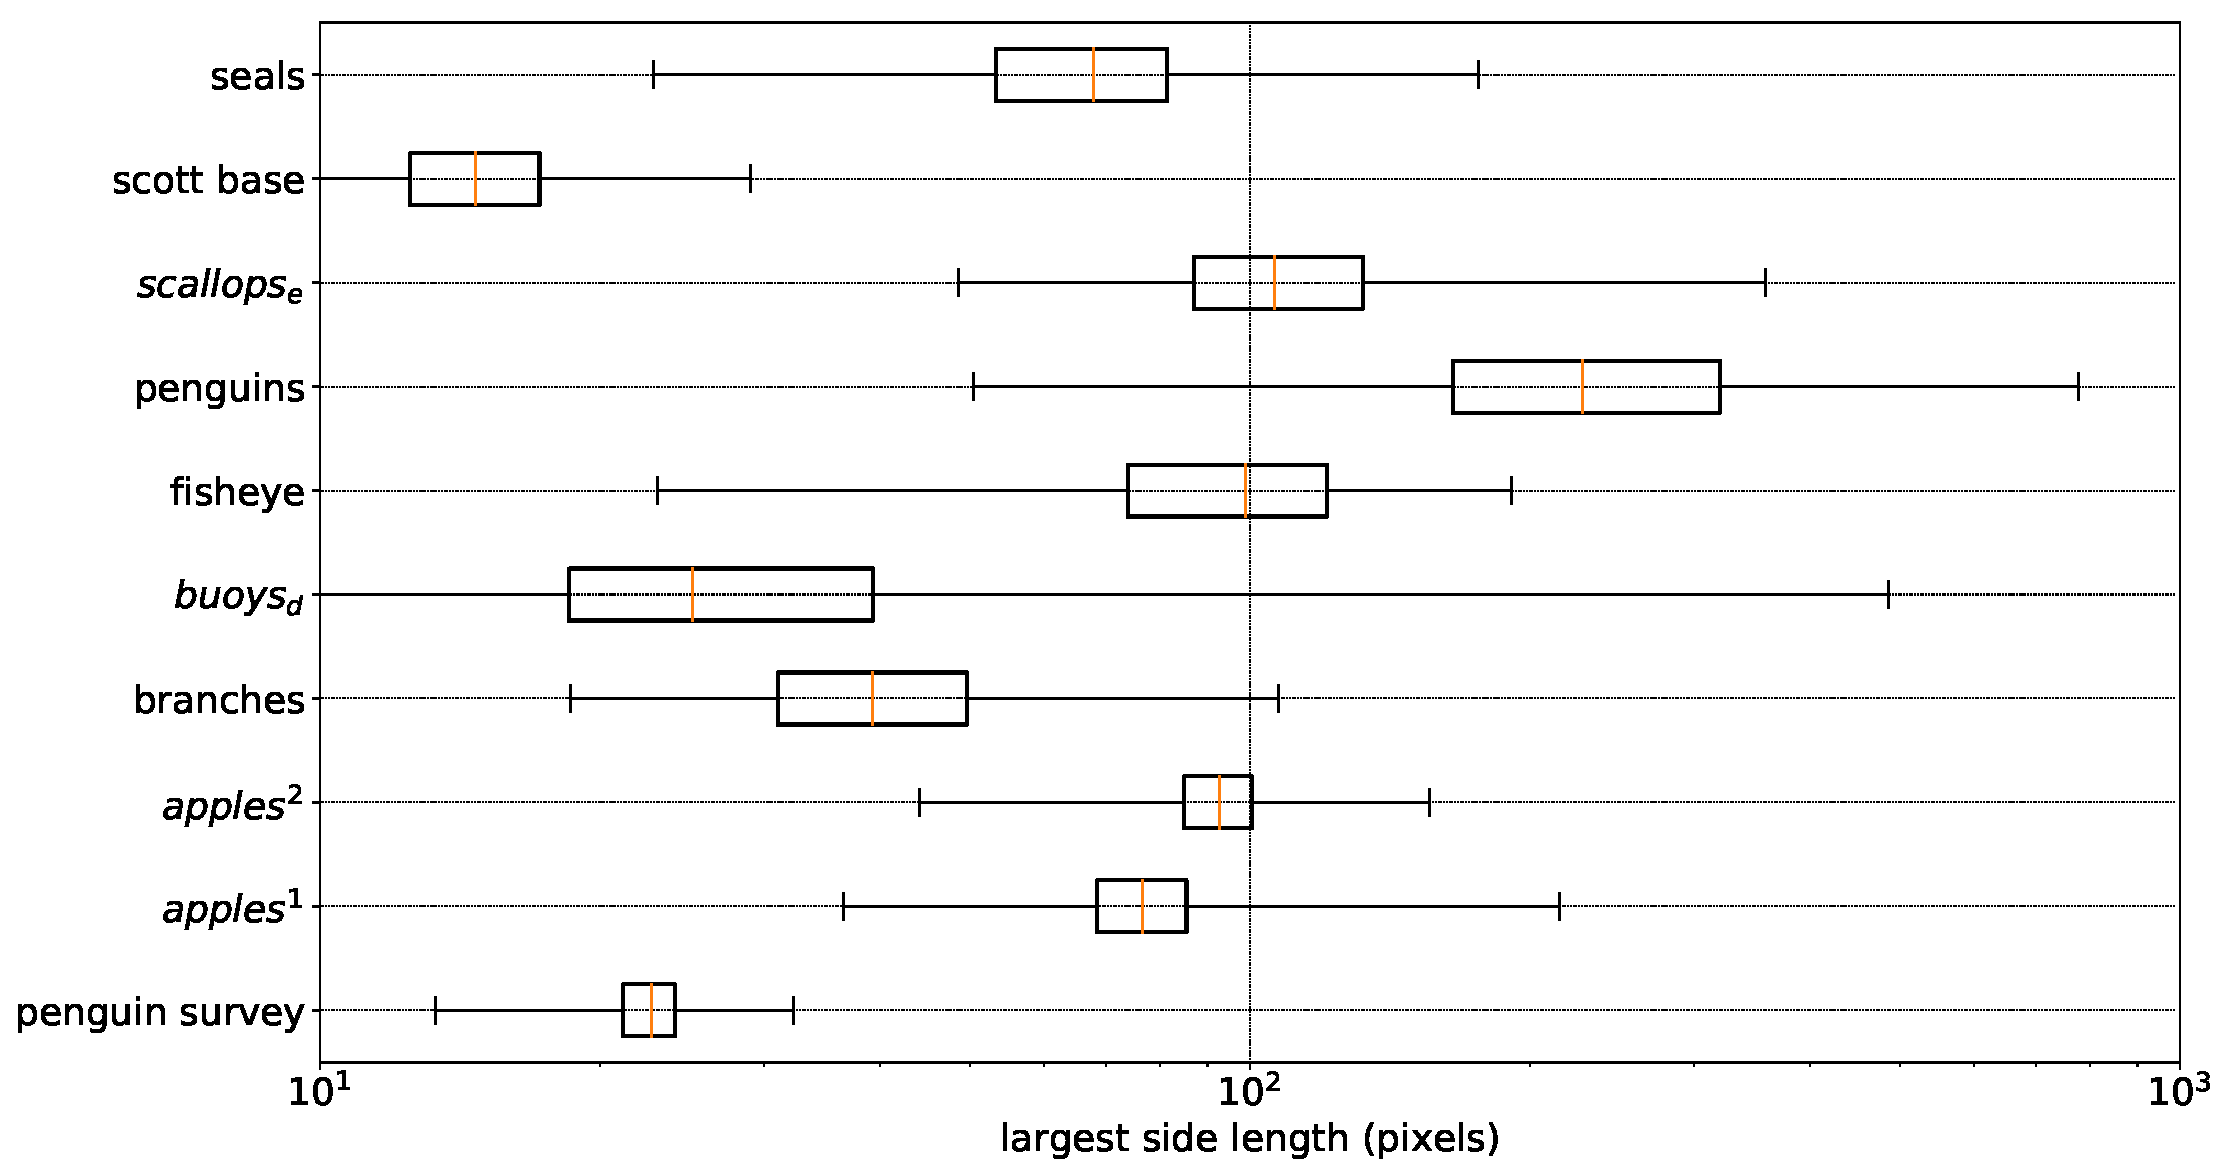
\includegraphics[width=1.0\linewidth]{charts/summaries/sizes_boxplot.pdf}
\caption{ Sizes in pixels of boxes for all annotated datasets }
\label{fig:box_sizes_plot}
\end{figure}

The sizes of objects in these datasets in general are small compared to more mainstream object detection datasets. This can be seen in figure~\ref{fig:box_sizes}, where compared to the Pascal VOC \cite{Everingham2008}, or COCO \cite{Lin2014}, the box sizes are smaller compared to the image size and less widely distributed. 

Figure \ref{fig:box_sizes_plot}  shows the object sizes (in pixels) of all the datasets together for comparison. In particular, the \emph{penguin survey} and \emph{scott base} datasets have particularly tiny objects (not shown on the figure in order to preserve the scale). It can be seen that although the box sizes are relatively small in terms of the relative size to the image that at full resolution the objects can be relatively large in pixels.

Two different types of annotations are used in the annotations of these datasets. Circular annotations are used for very small objects and for counting objects where precise localisation is of less concern; circular annotations are also used for apples where it just happens to match the object shape well. The difference to the object detector is that a centre and radius is estimated (instead of centre, width and height). The circles are treated as a square for computations such as \gls{IOU} overlap.

\subsection {Instance distribution}

\begin{figure}[ht]
\centering
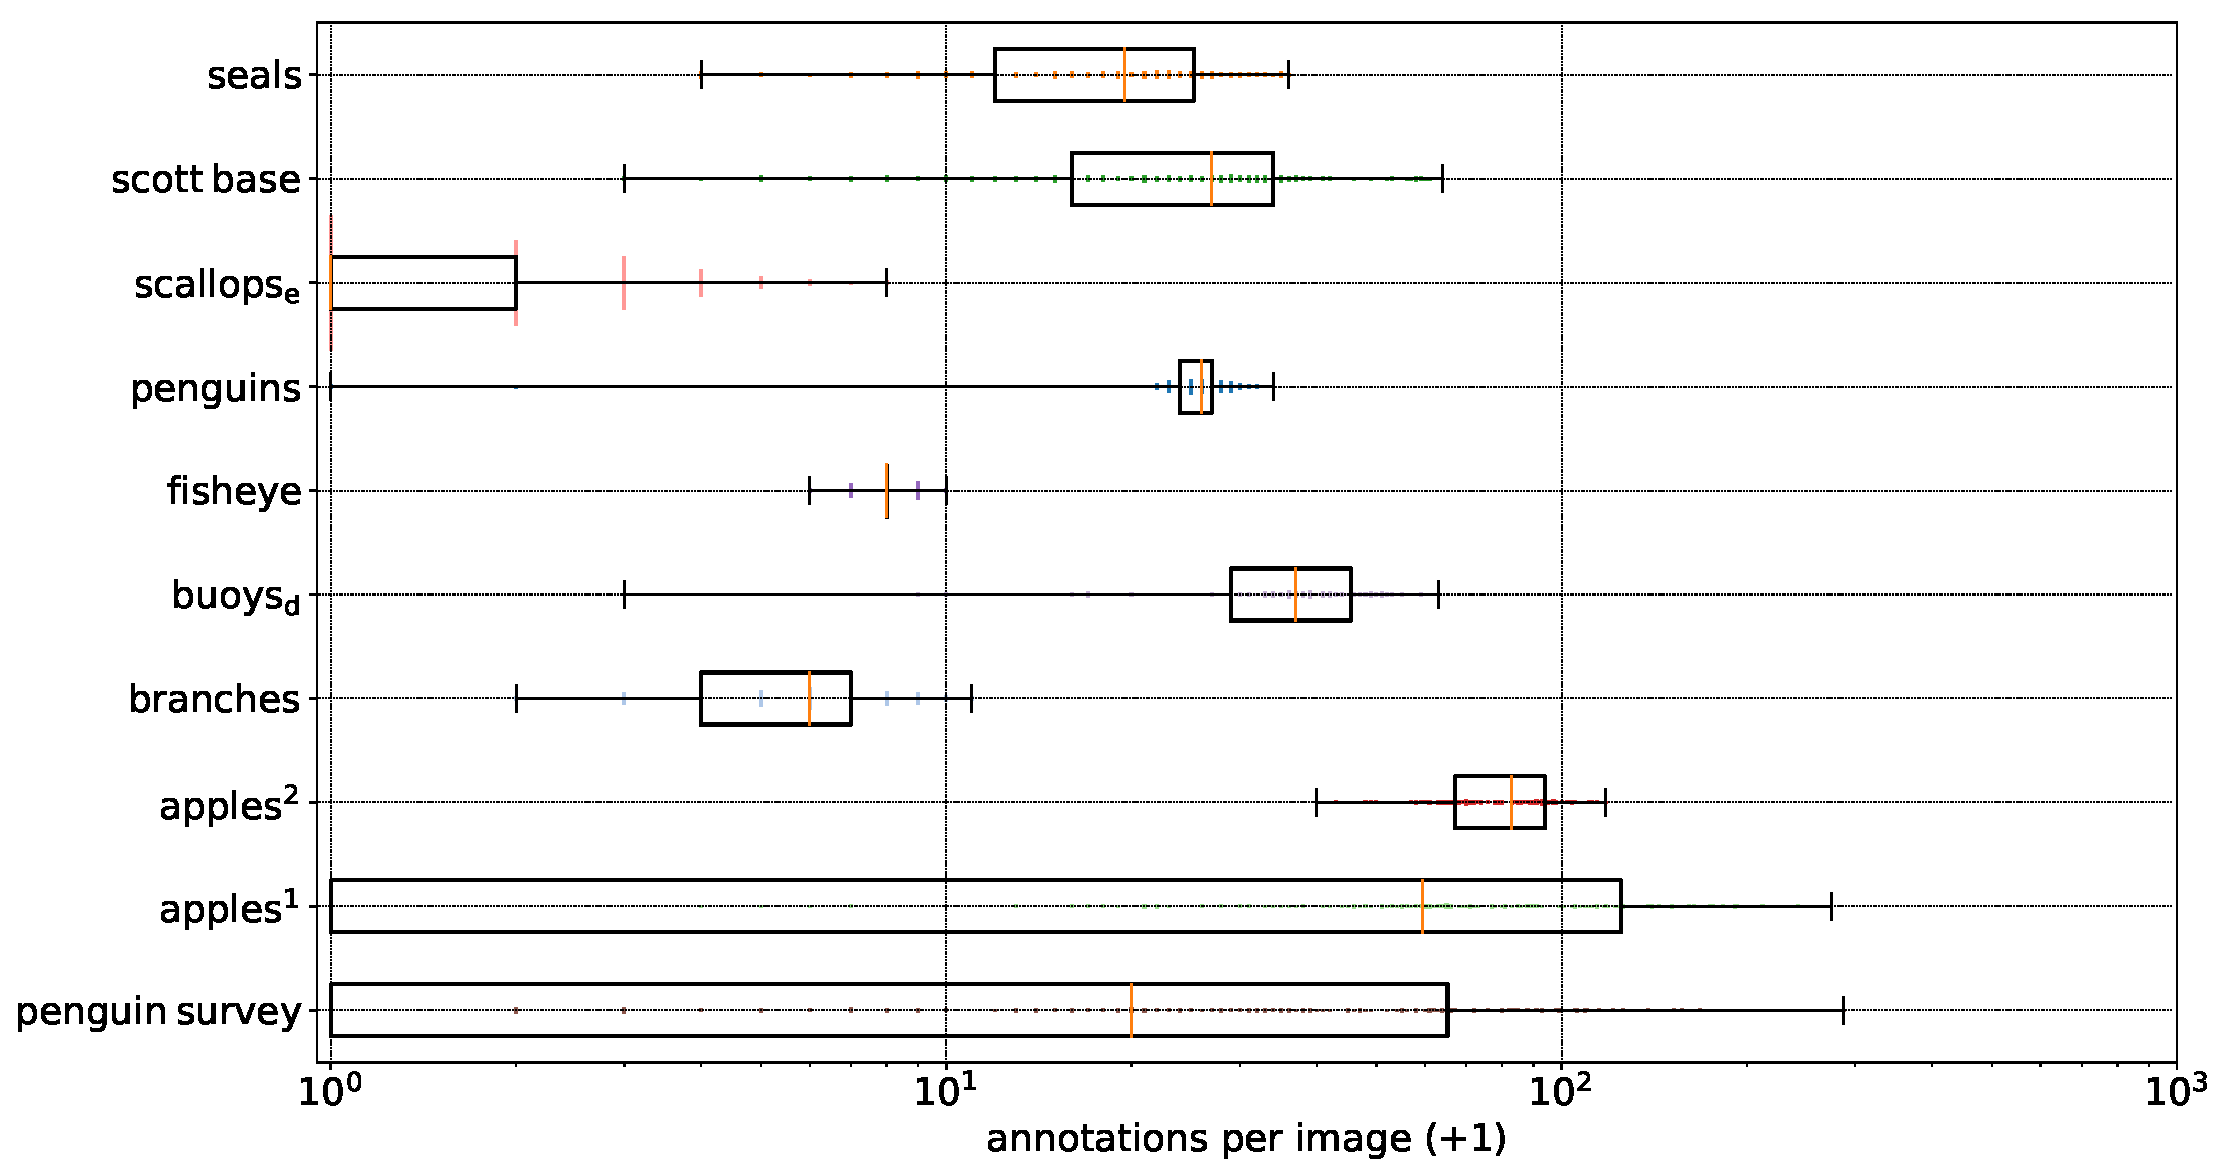
\includegraphics[width=1.0\linewidth]{charts/summaries/instances_boxplot.pdf}
\caption{ Distribution of object annotations per image }
\label{fig:instances_image_plot}
\end{figure}

The datasets in question have a wide range of instance distributions, shown in figure~\ref{fig:instances_image_plot}. Some such as \emph{apples2}, \emph{branches} and \emph{fisheye} and \emph{penguins} contain a relatively uniform numbers of annotations. Others especially \emph {penguin surveys}, \emph{scott base} and \emph{apples1} contain a wide range, a few with several hundred annotations per image. One, \emph{scallops} contains very few annotations ($0.54$ per image), where most images are negative images.


\subsection {Actions and corrections}

\begin{figure}[H] 
\centering
\begin{subfigure}{0.48\linewidth}
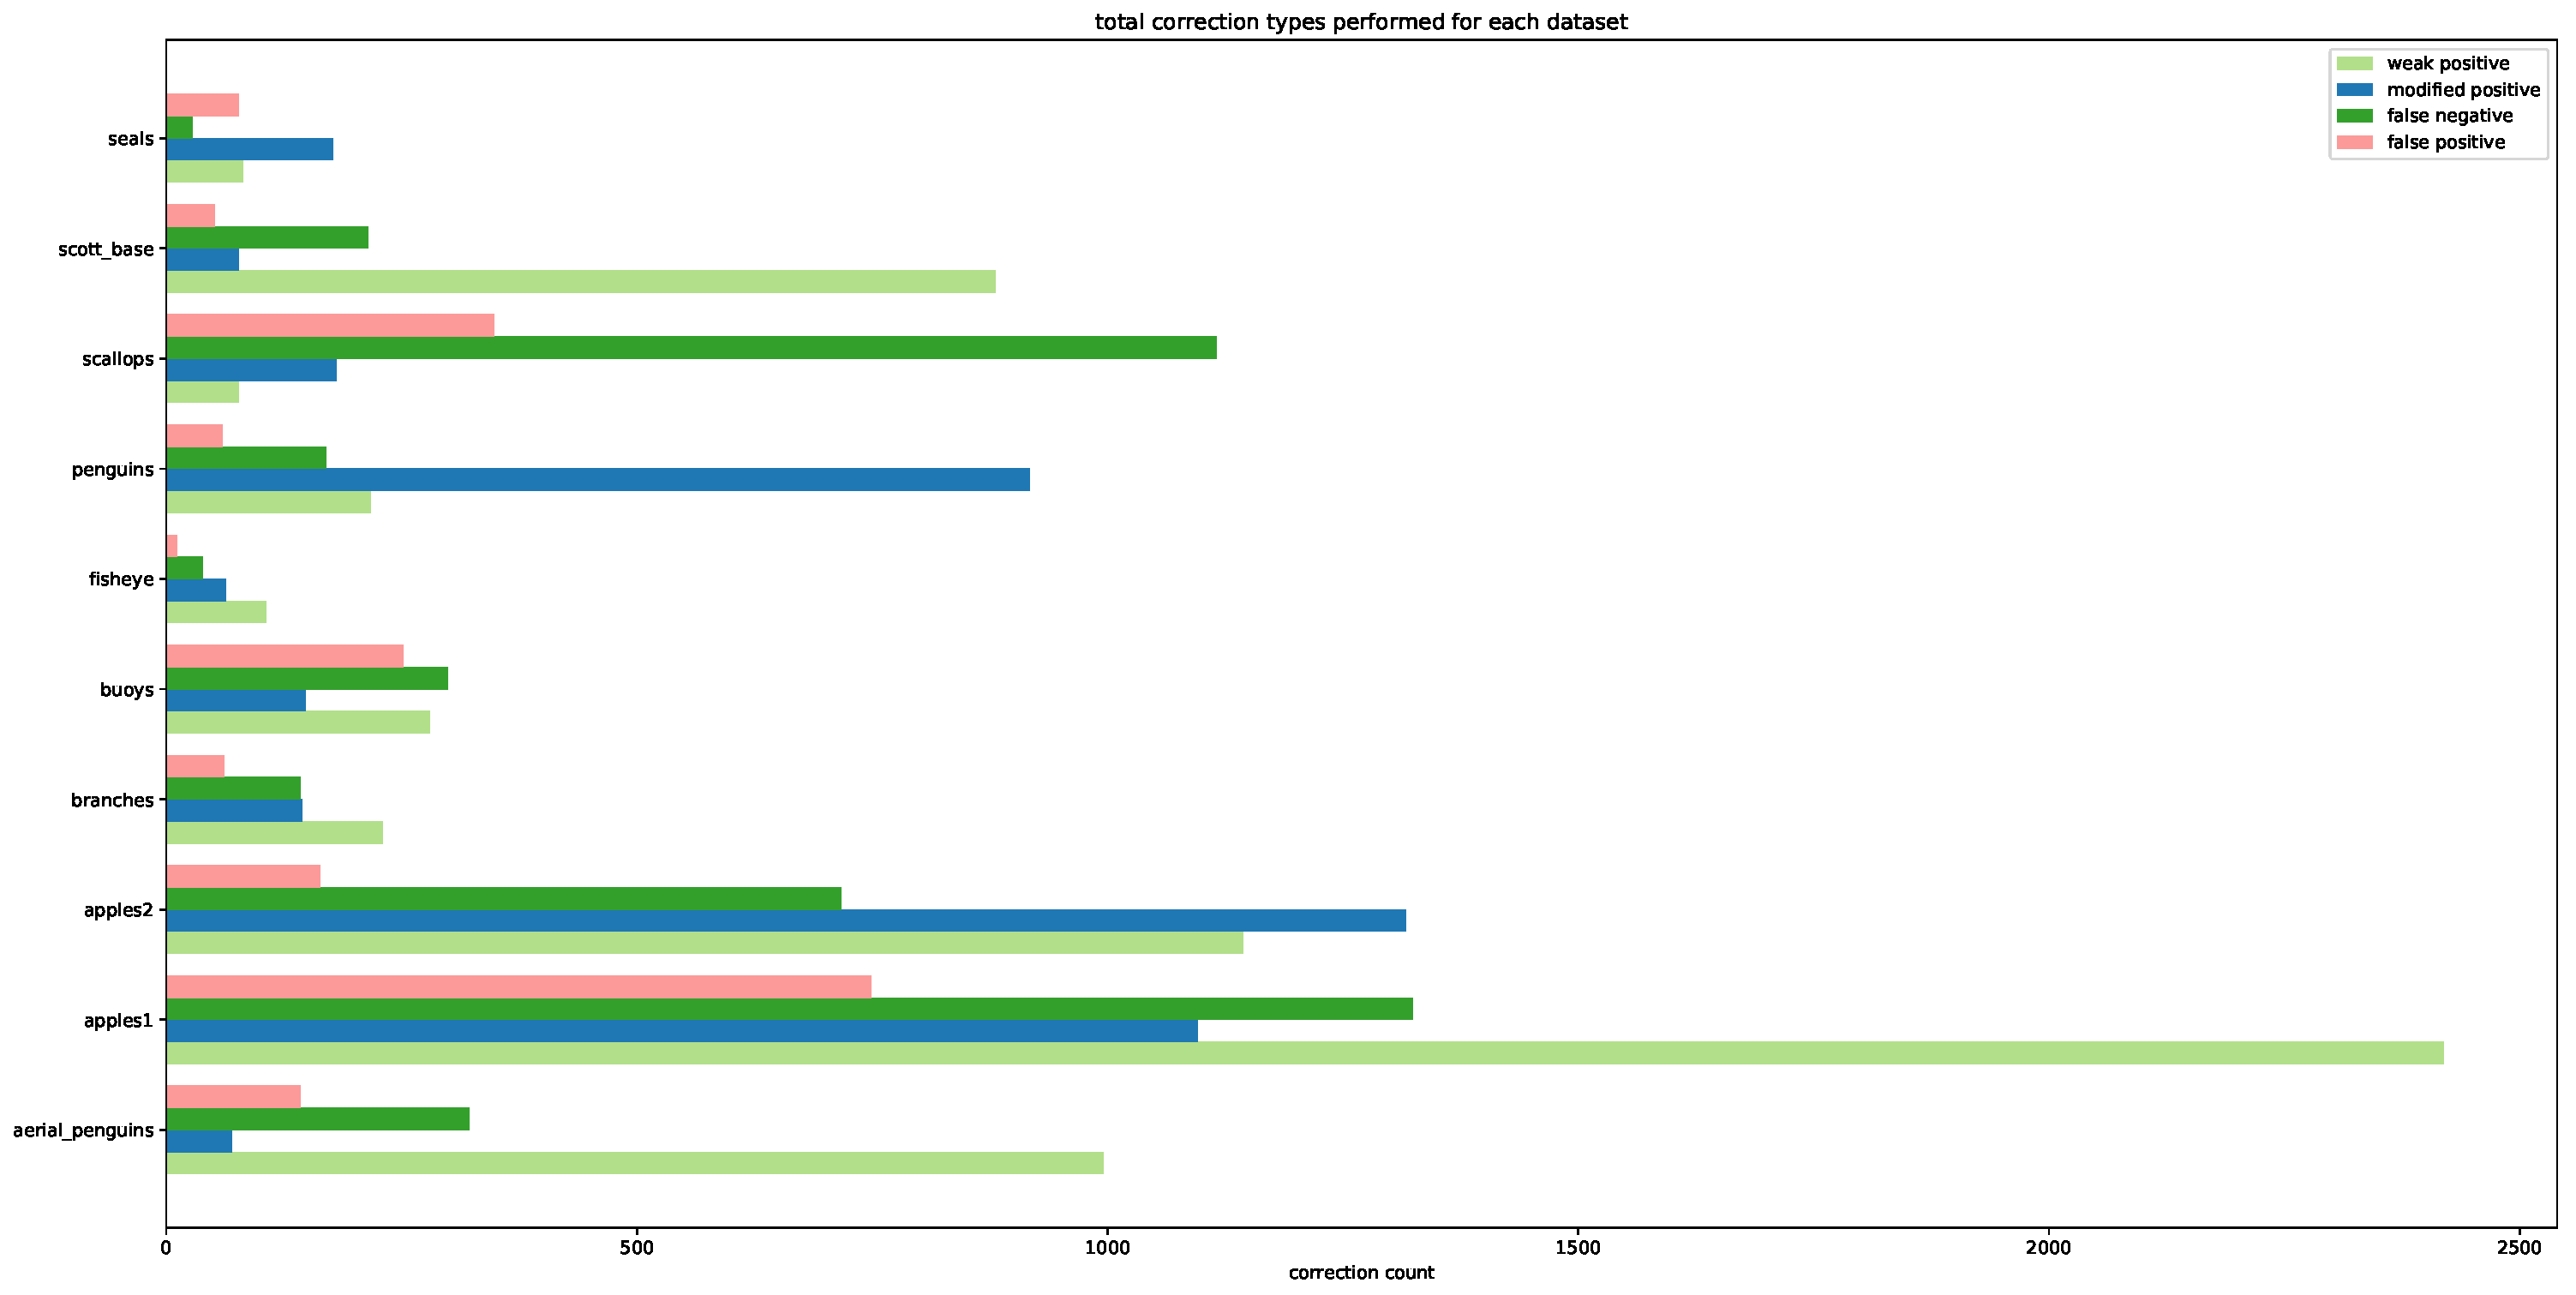
\includegraphics[width=1.0\linewidth]{charts/summaries/correction_counts.pdf}
\caption{Corrected annotation types as a proportion of final annotation count}
\end{subfigure}%
\begin{subfigure}{0.48\linewidth}
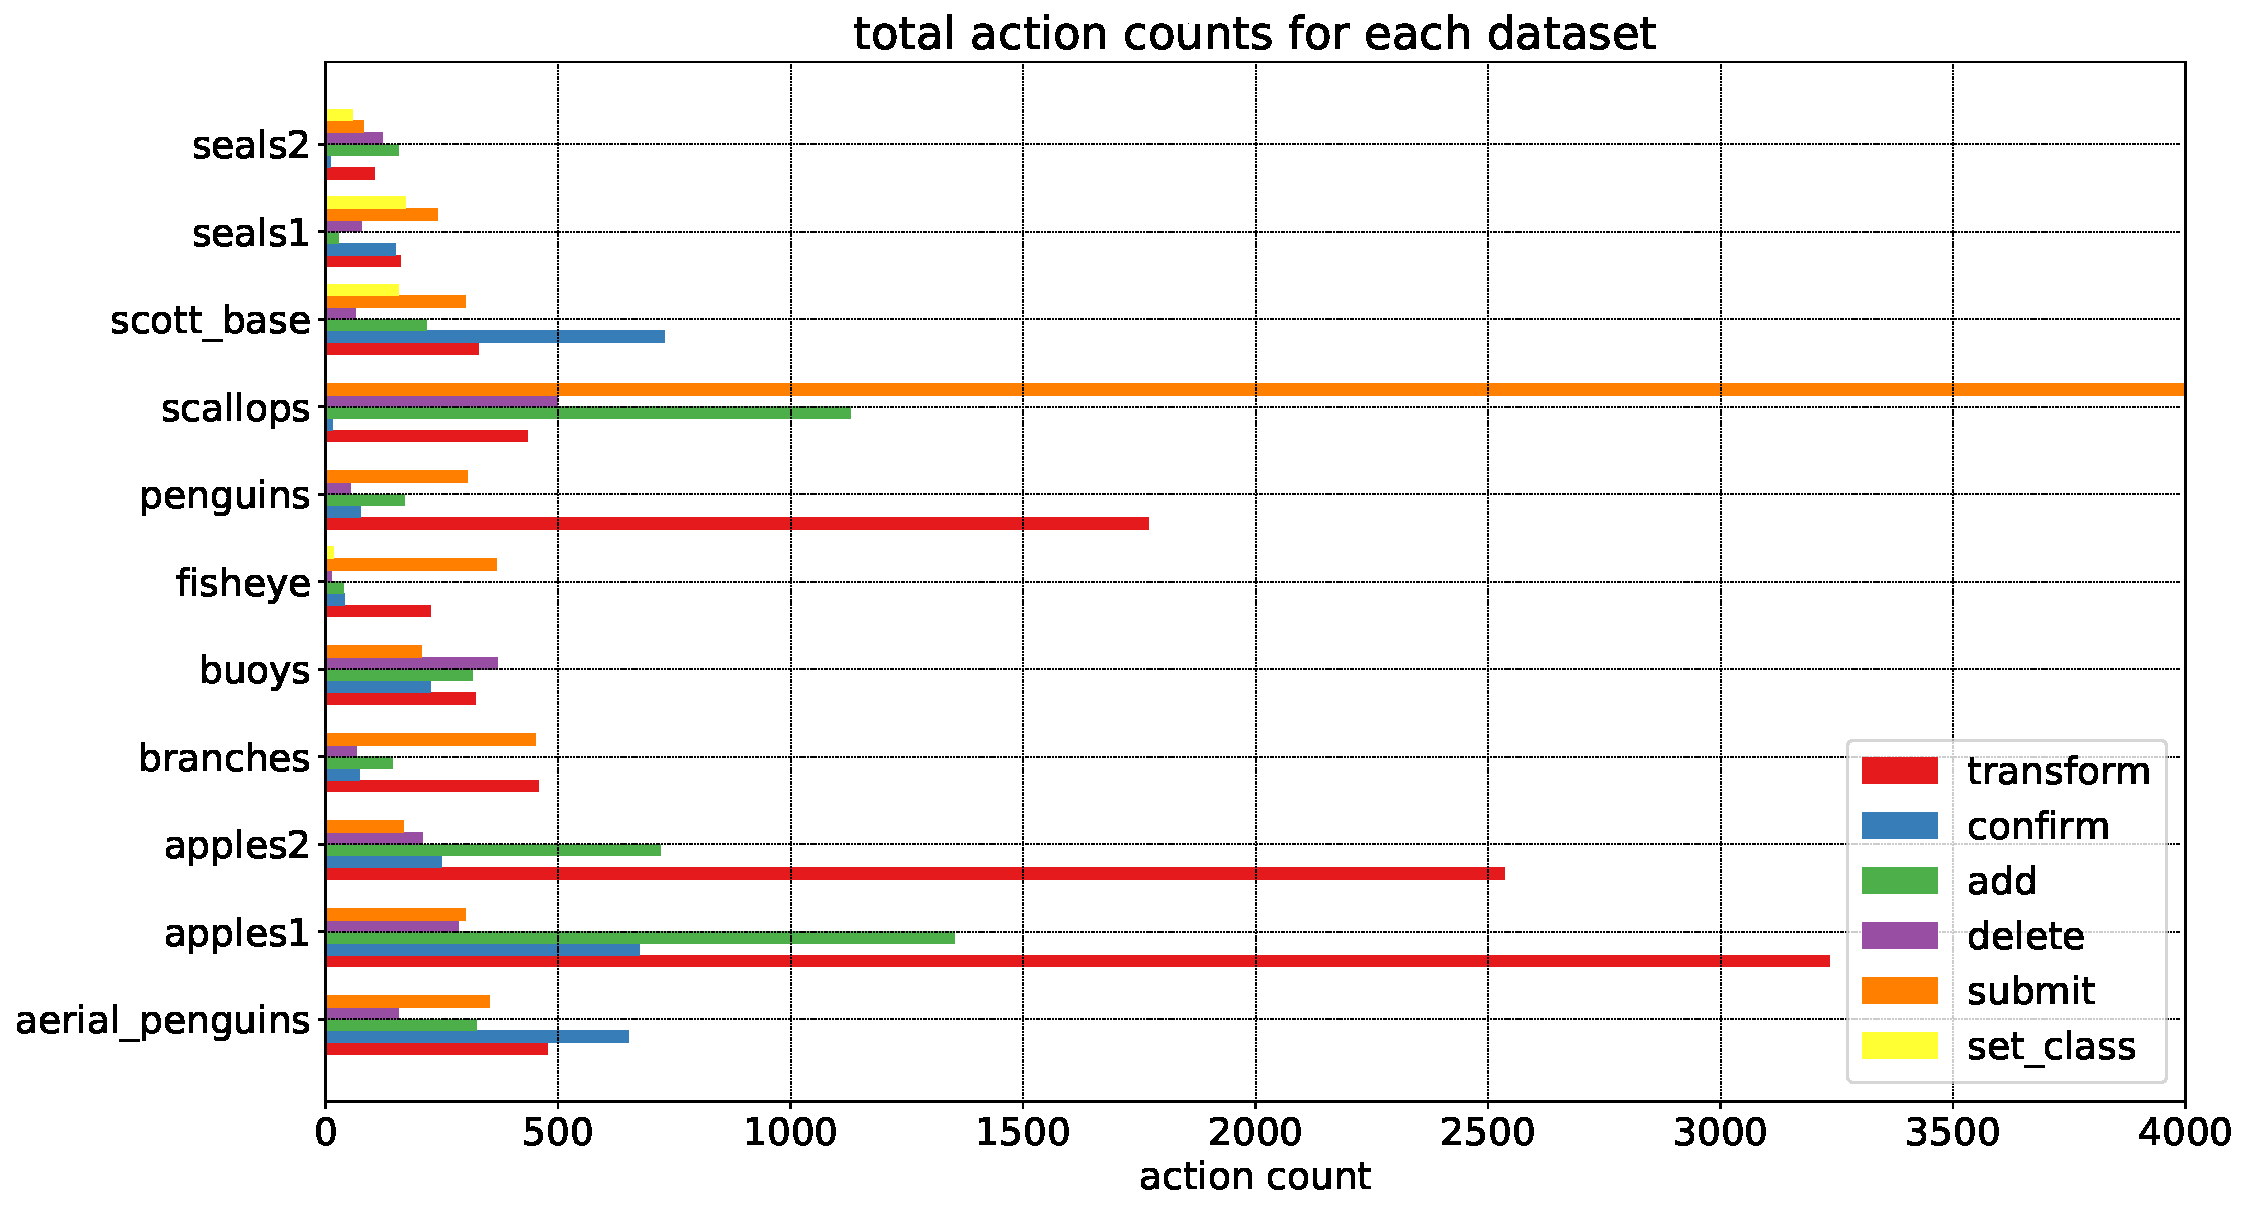
\includegraphics[width=1.0\linewidth]{charts/summaries/action_counts.pdf} 
\caption{Proportions of actions}
\end{subfigure}

\label{fig:actions_dataset}
\end{figure}





\begin{figure}[ht]
\centering
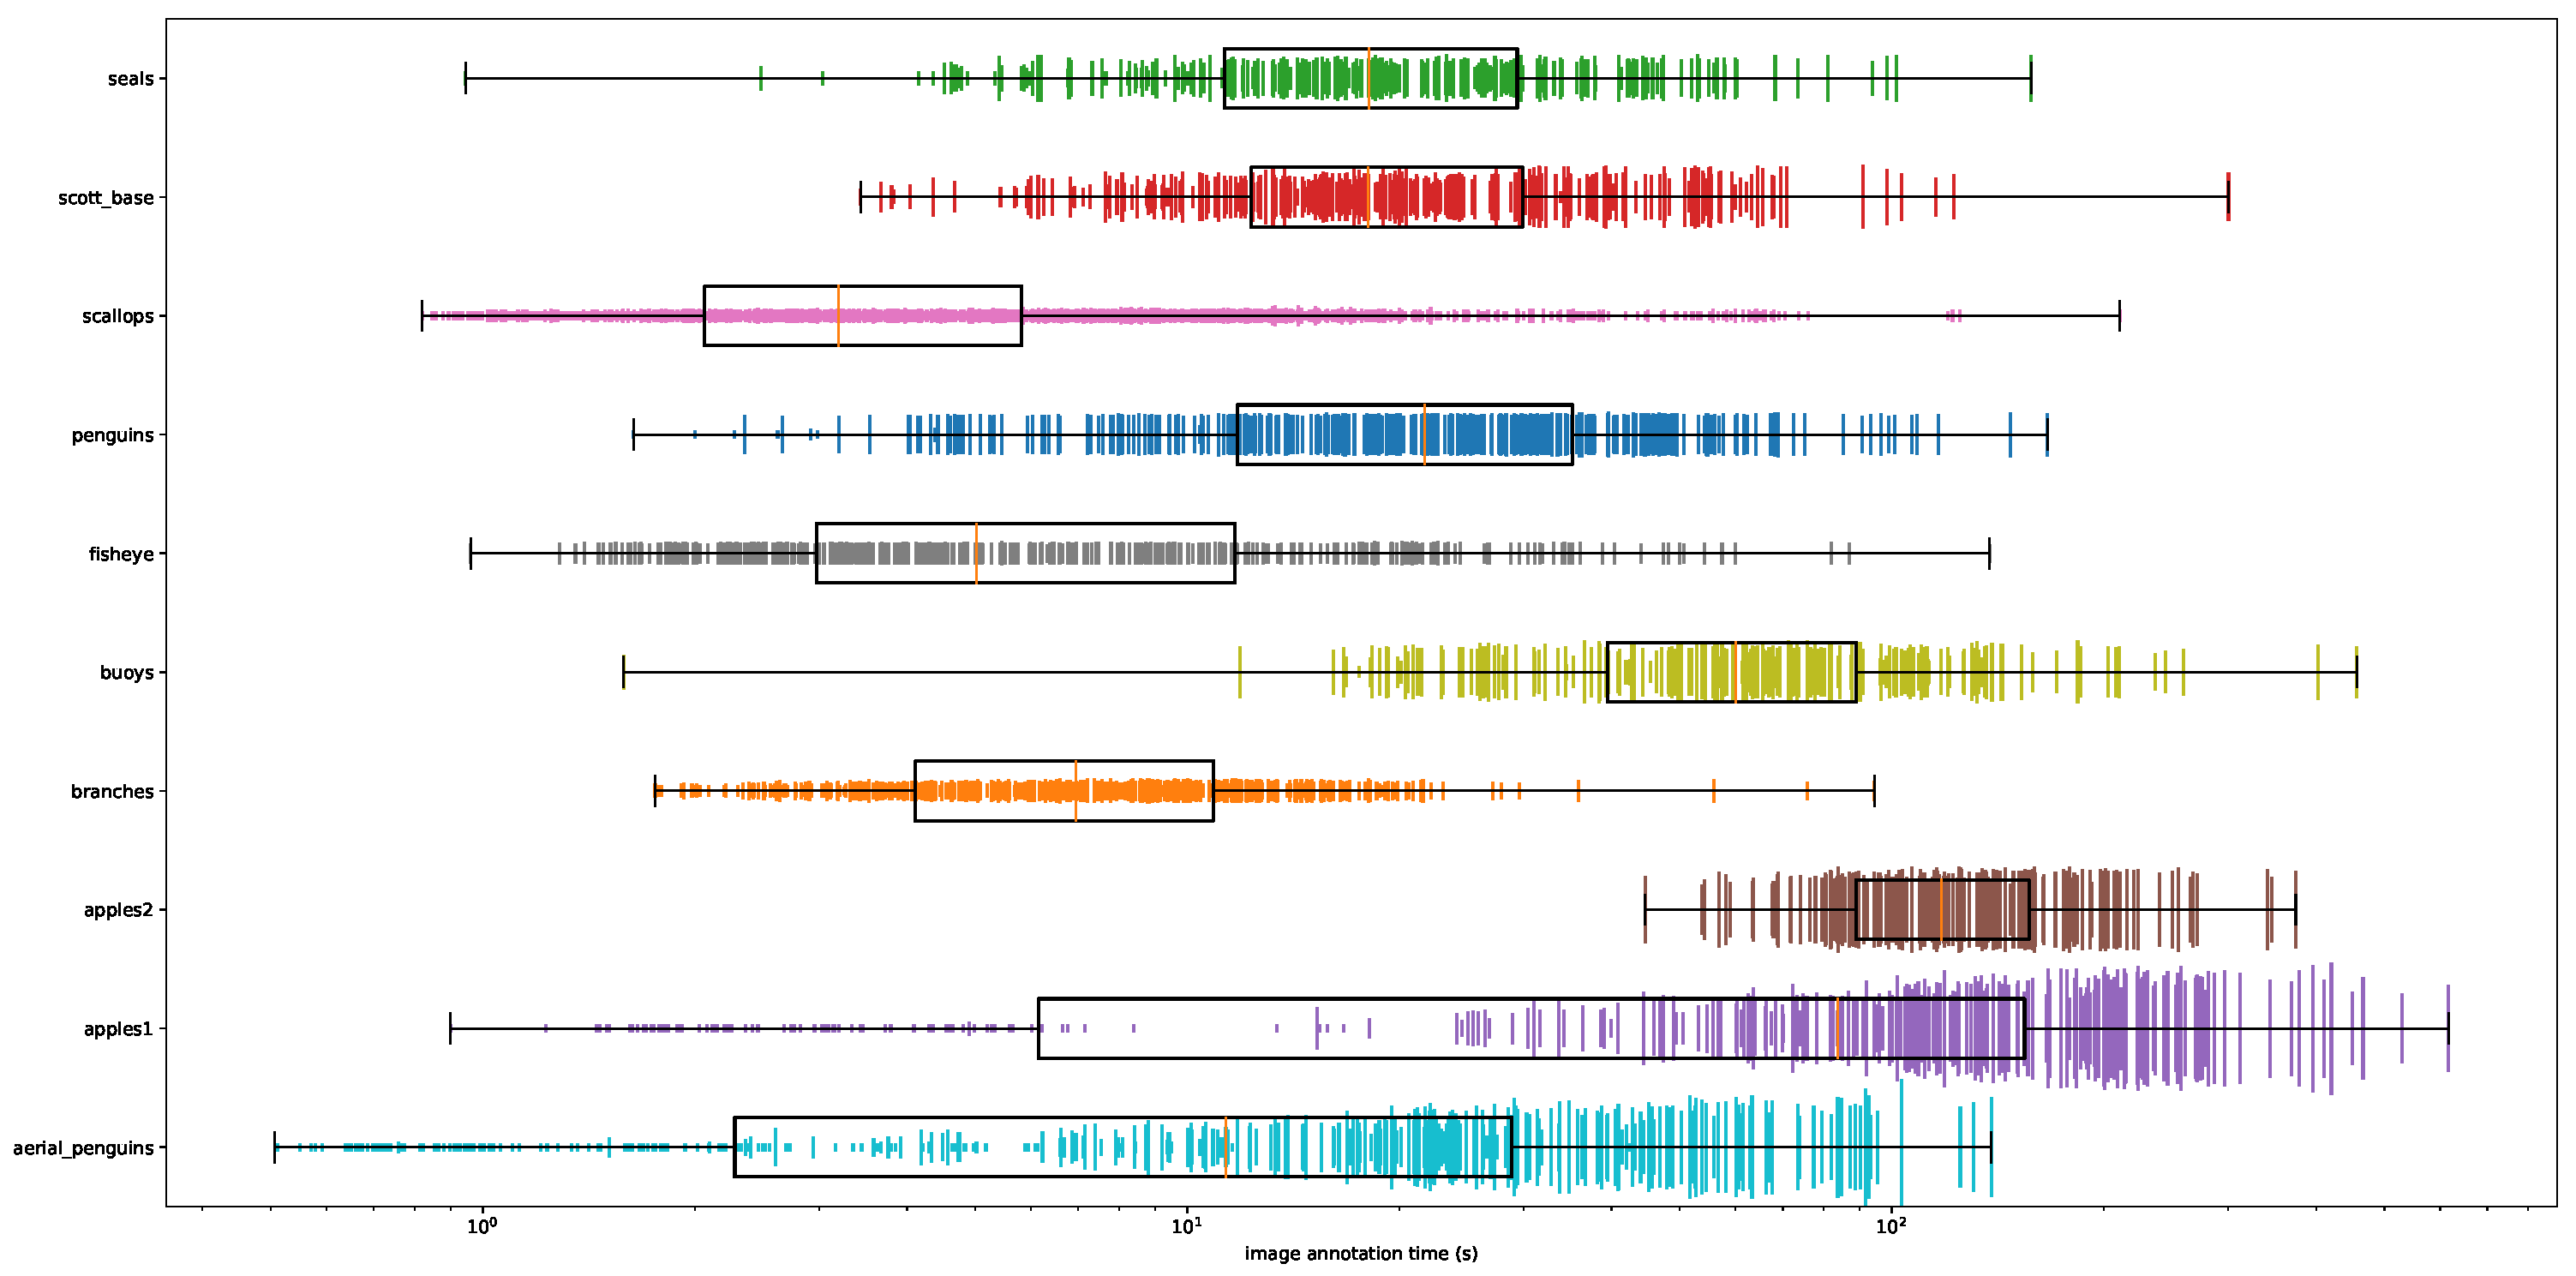
\includegraphics[width=1.0\linewidth]{charts/summaries/duration_boxplot.pdf}
\caption{ Per image annotation time distributions, vertical lines show the individual images and the height of each line is proportional to the square root of number of instances }
\label{fig:duration_boxplot}
\end{figure}




\subsection{Annotation rate}

\begin{figure}[H]
\centering
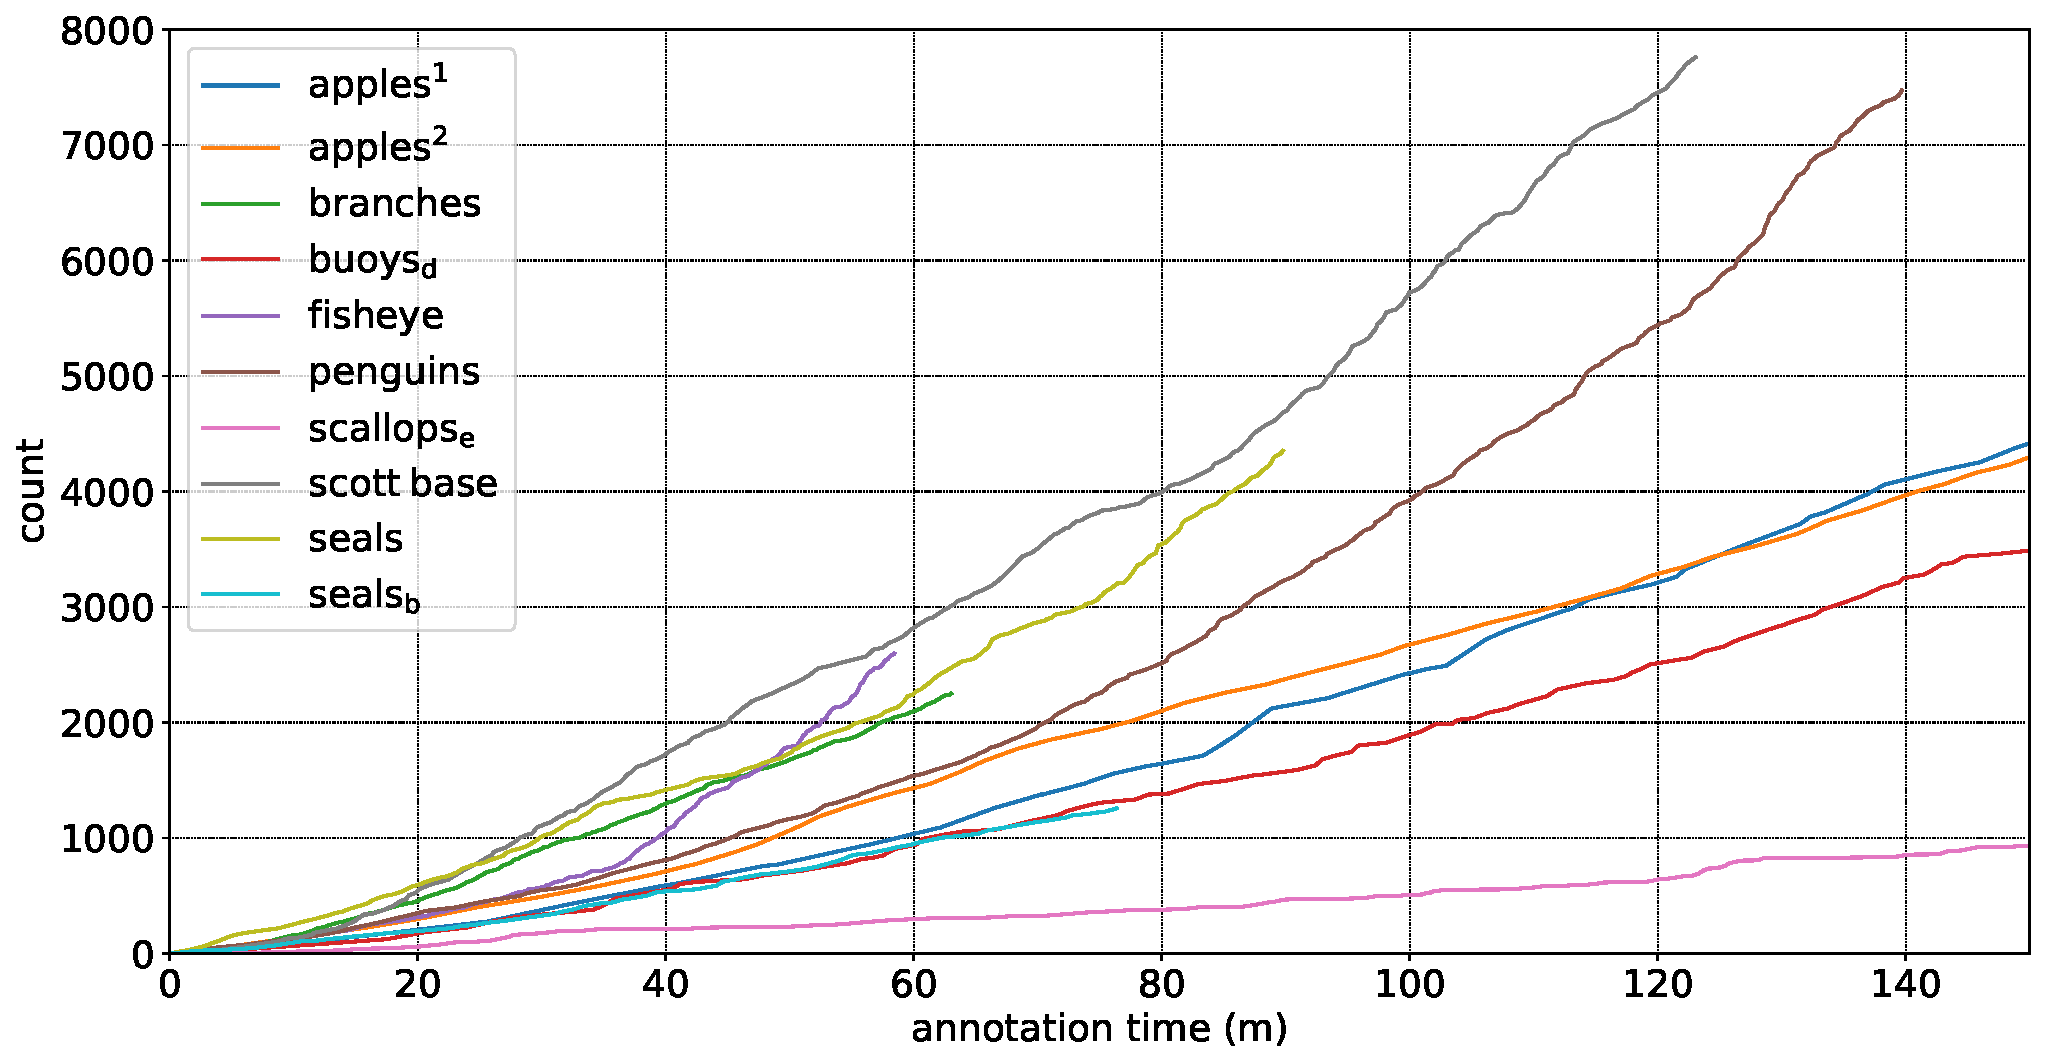
\includegraphics[width=1.0\linewidth]{charts/summaries/cumulative_instances_crop.pdf}
\caption{ Cumulative instances annotated (truncated to first 140 minutes)  }
\label{fig:cumulative_instances}
\end{figure}



\begin{figure}[H]
\centering
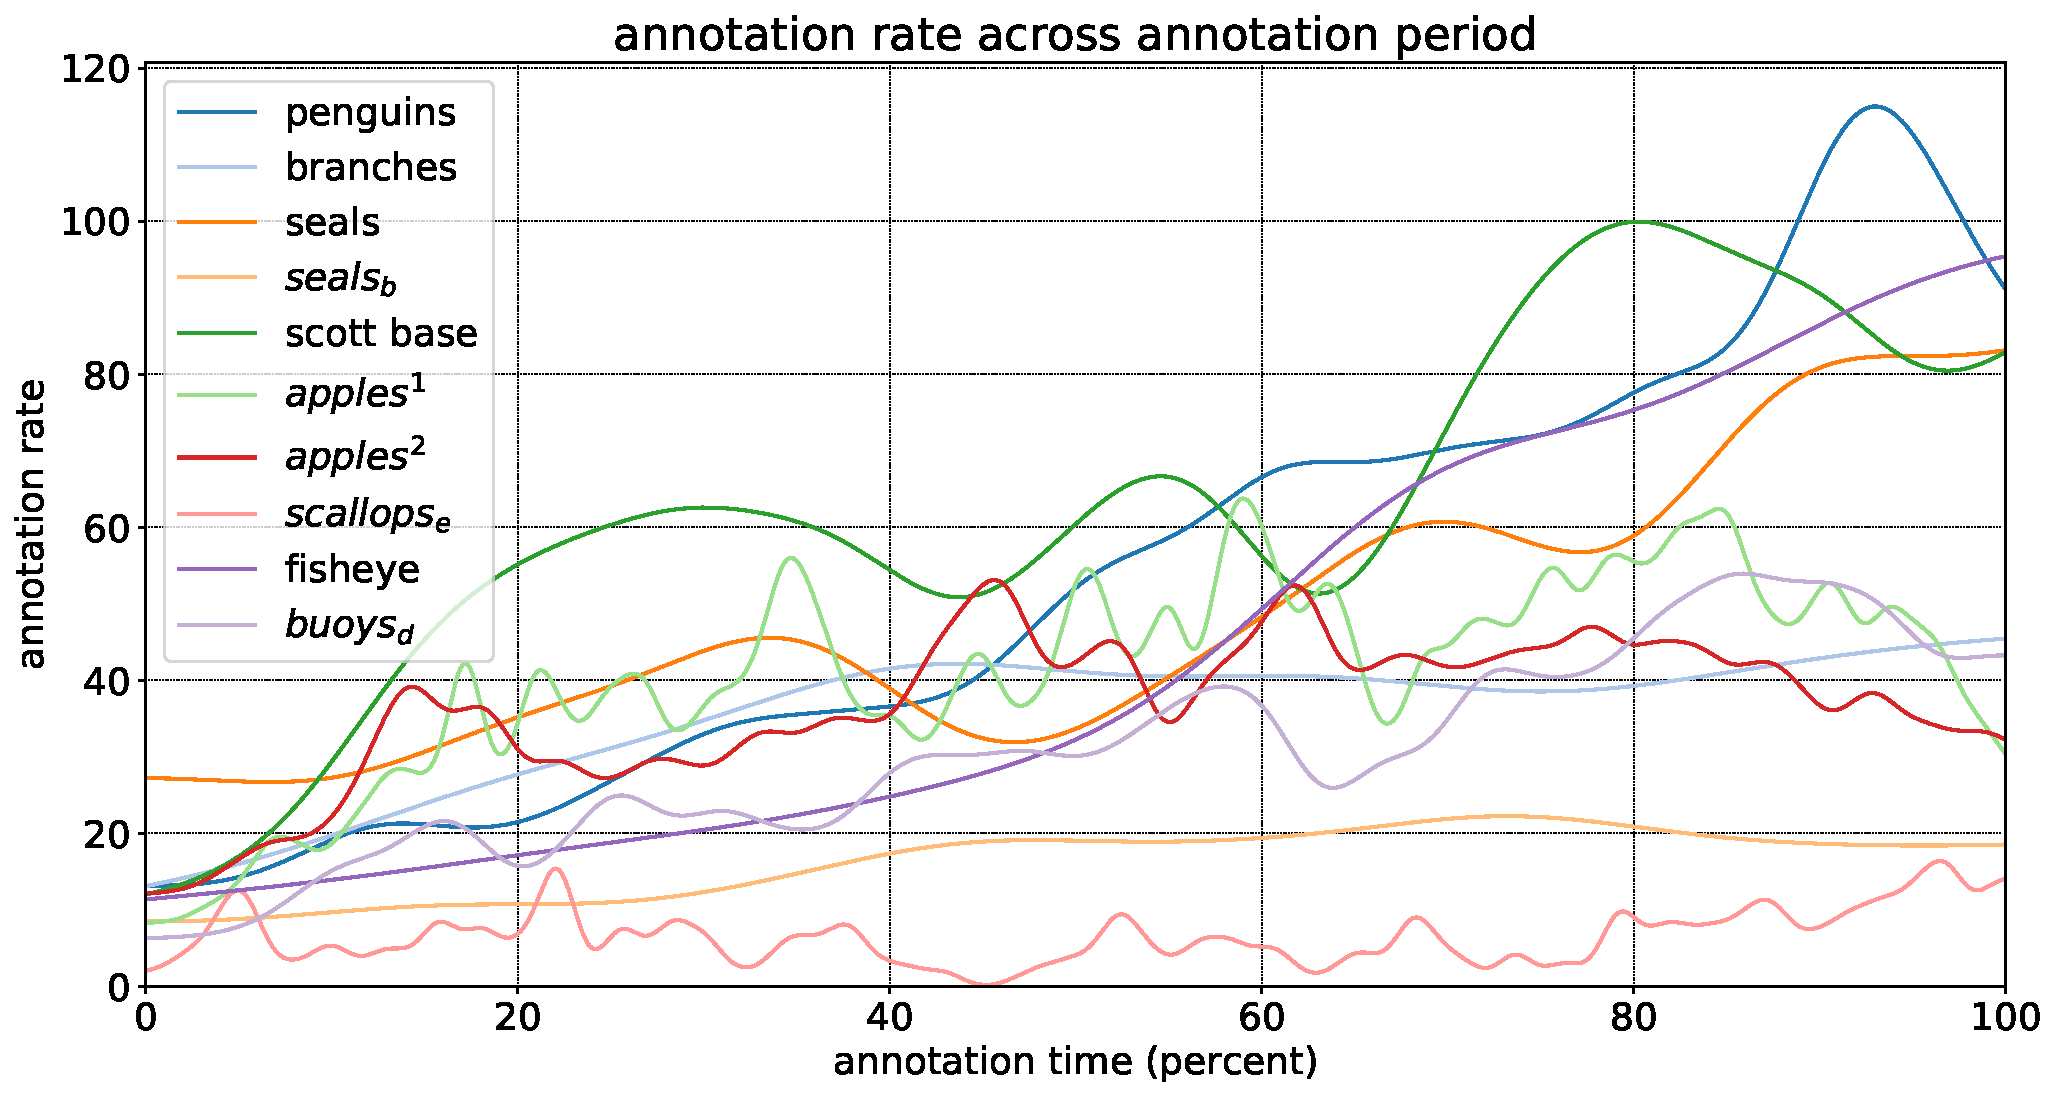
\includegraphics[width=1.0\linewidth]{charts/summaries/instance_rates.pdf}
\caption{ Annotation rate for all datasets (instances per minute) across annotation period, density plot with $\sigma=5minutes$ }
\label{fig:annotation_rate}
\end{figure}




\subsection{Continuous testing: object detection accuracy}
\label{sec:continuous_testing}

\begin{figure}[H]
\centering
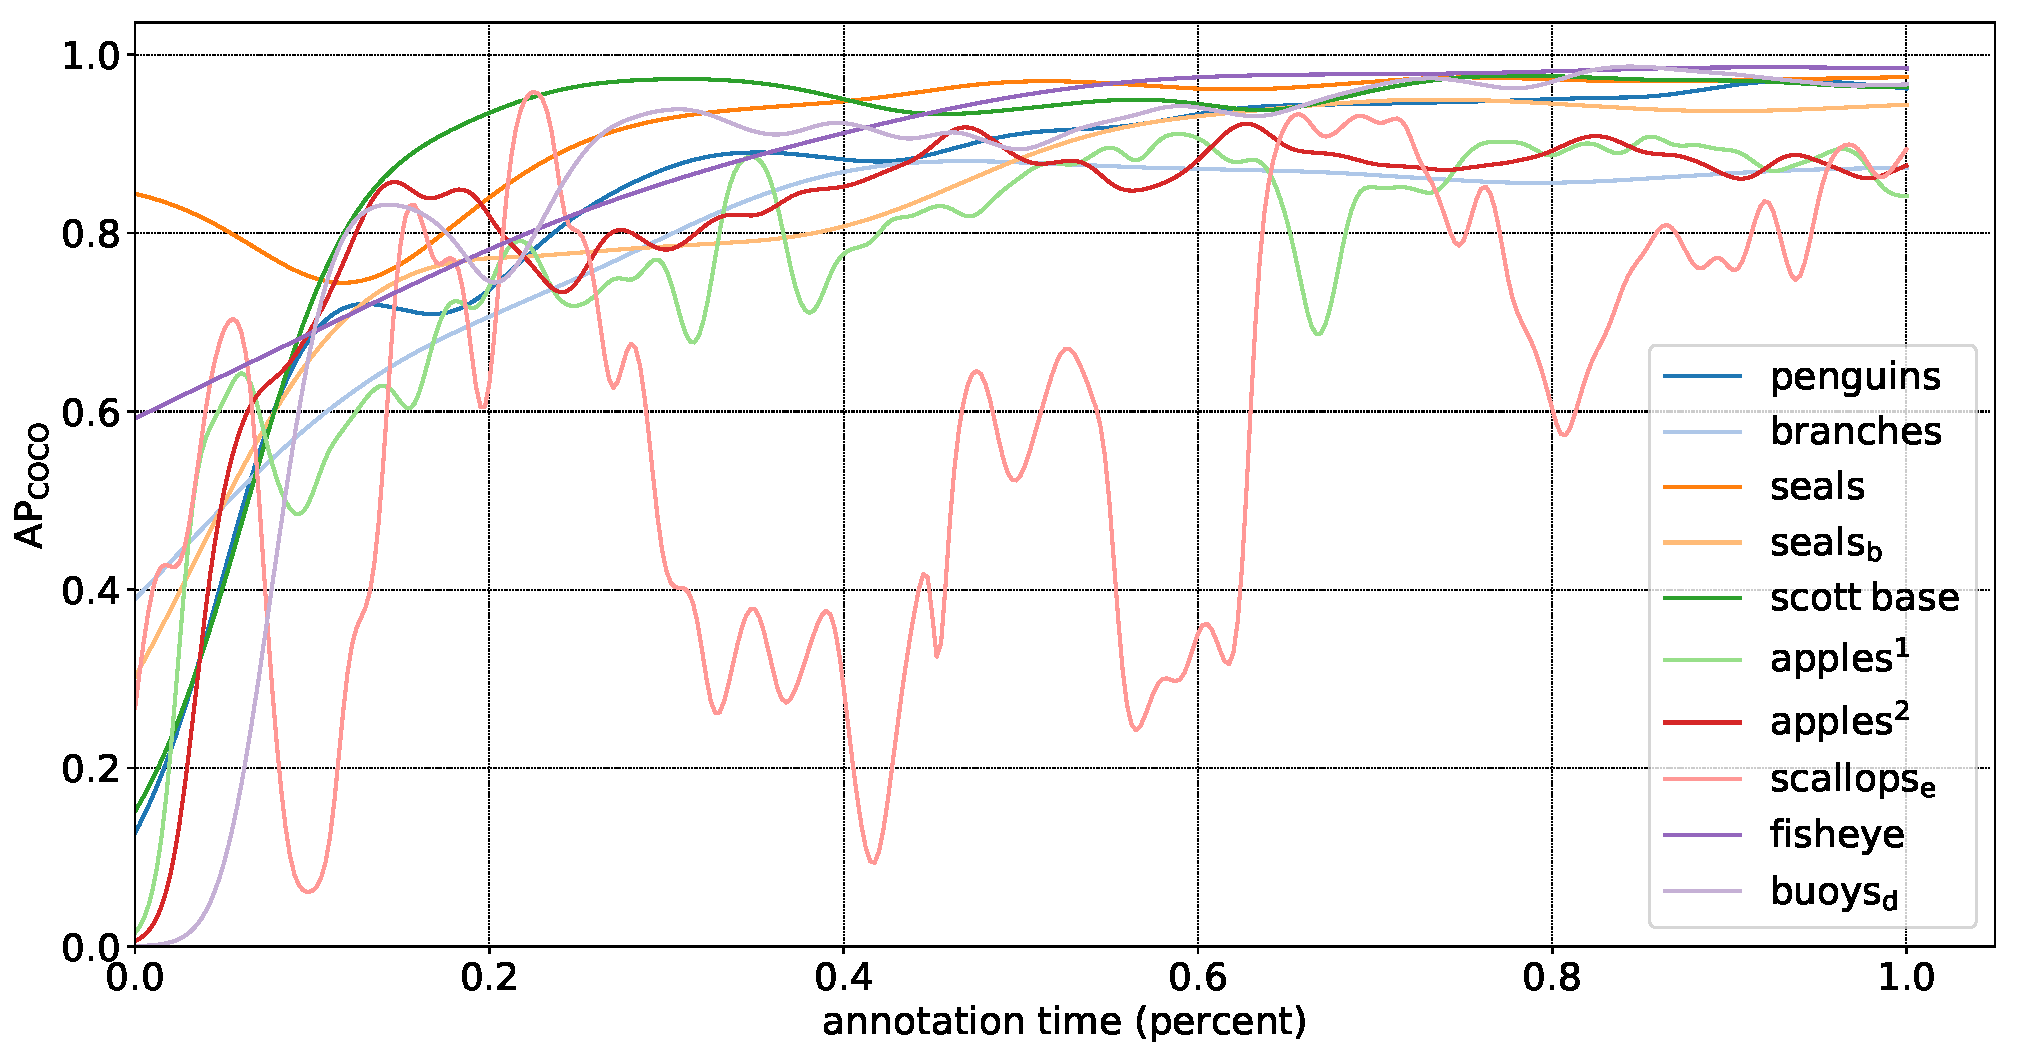
\includegraphics[width=1.0\linewidth]{charts/running_maps/overall.pdf}
\caption{ Local $AP_{COCO}$ of detections with respect to corrected annotations }
\label{fig:average_precision_test}
\end{figure}

Figure~\ref{fig:average_precision_test} shows the locally weighted average precision for each dataset across annotation time, providing a single metric to describe the level of assistance provided to the human annotator. 

It can be seen for example that the reason for the dips in the annotation rate for the \emph{scallops} dataset is not solely because of sparsity of the scallop instances in the images annotated at that point in time, but also a dip in object detection accuracy on those images.


\subsection{Localisation precision}
\label{sec:localisation_precision}


One aspect of note is that there exists a gap between the $AP_{COCO}$ reported in figure~\ref{fig:average_precision_test} and the $AP_{COCO}$ from testing the object detector against it's validation set seen in figure~\ref{fig:validation}. The validation set accuracy is much lower in all cases, the reason for this is that the human threshold for acceptance is lower. 

There exists a tolerance threshold for a human annotator using verification based annotation this threshold can be seen indirectly in figure~\ref{fig:density_iou} where the density of transformed detections peaks at around $0.80$--$0.85$ depending on the dataset (for the \emph{penguin survey} it is lower, where counting was emphasised over precise localisation). At higher \gls{IOU} levels this drops off, showing that at that point the annotations match an acceptable level of error according to the human annotator. 

You would expect that the actual localisation error distribution would be much more smooth with no gap and also no perfectly accurate object detections.
 
The \gls{AP} metric has some systematic differences when applied this way, meaning it is not comparable with the testing on the validation set for example. If an detection is accepted \emph{as is} by the human annotator it is considered to be $100\%$ precise (even at $0.95$ \gls{IOU} threshold), where as if a human was to draw a box it would match the predicted box at that level of accuracy with much lower probability. 

On the other hand it could be argued that the metric created from human corrections was the better one, simply because it does include that level of tolerance. Where the scoring calculated from testing on the validation set may penalise tiny differences; the score based on human corrections takes into account the desired level of localisation precision, and small differences because of uncertainty or irrelevant details are ignored.


\begin{figure}[ht]
\centering
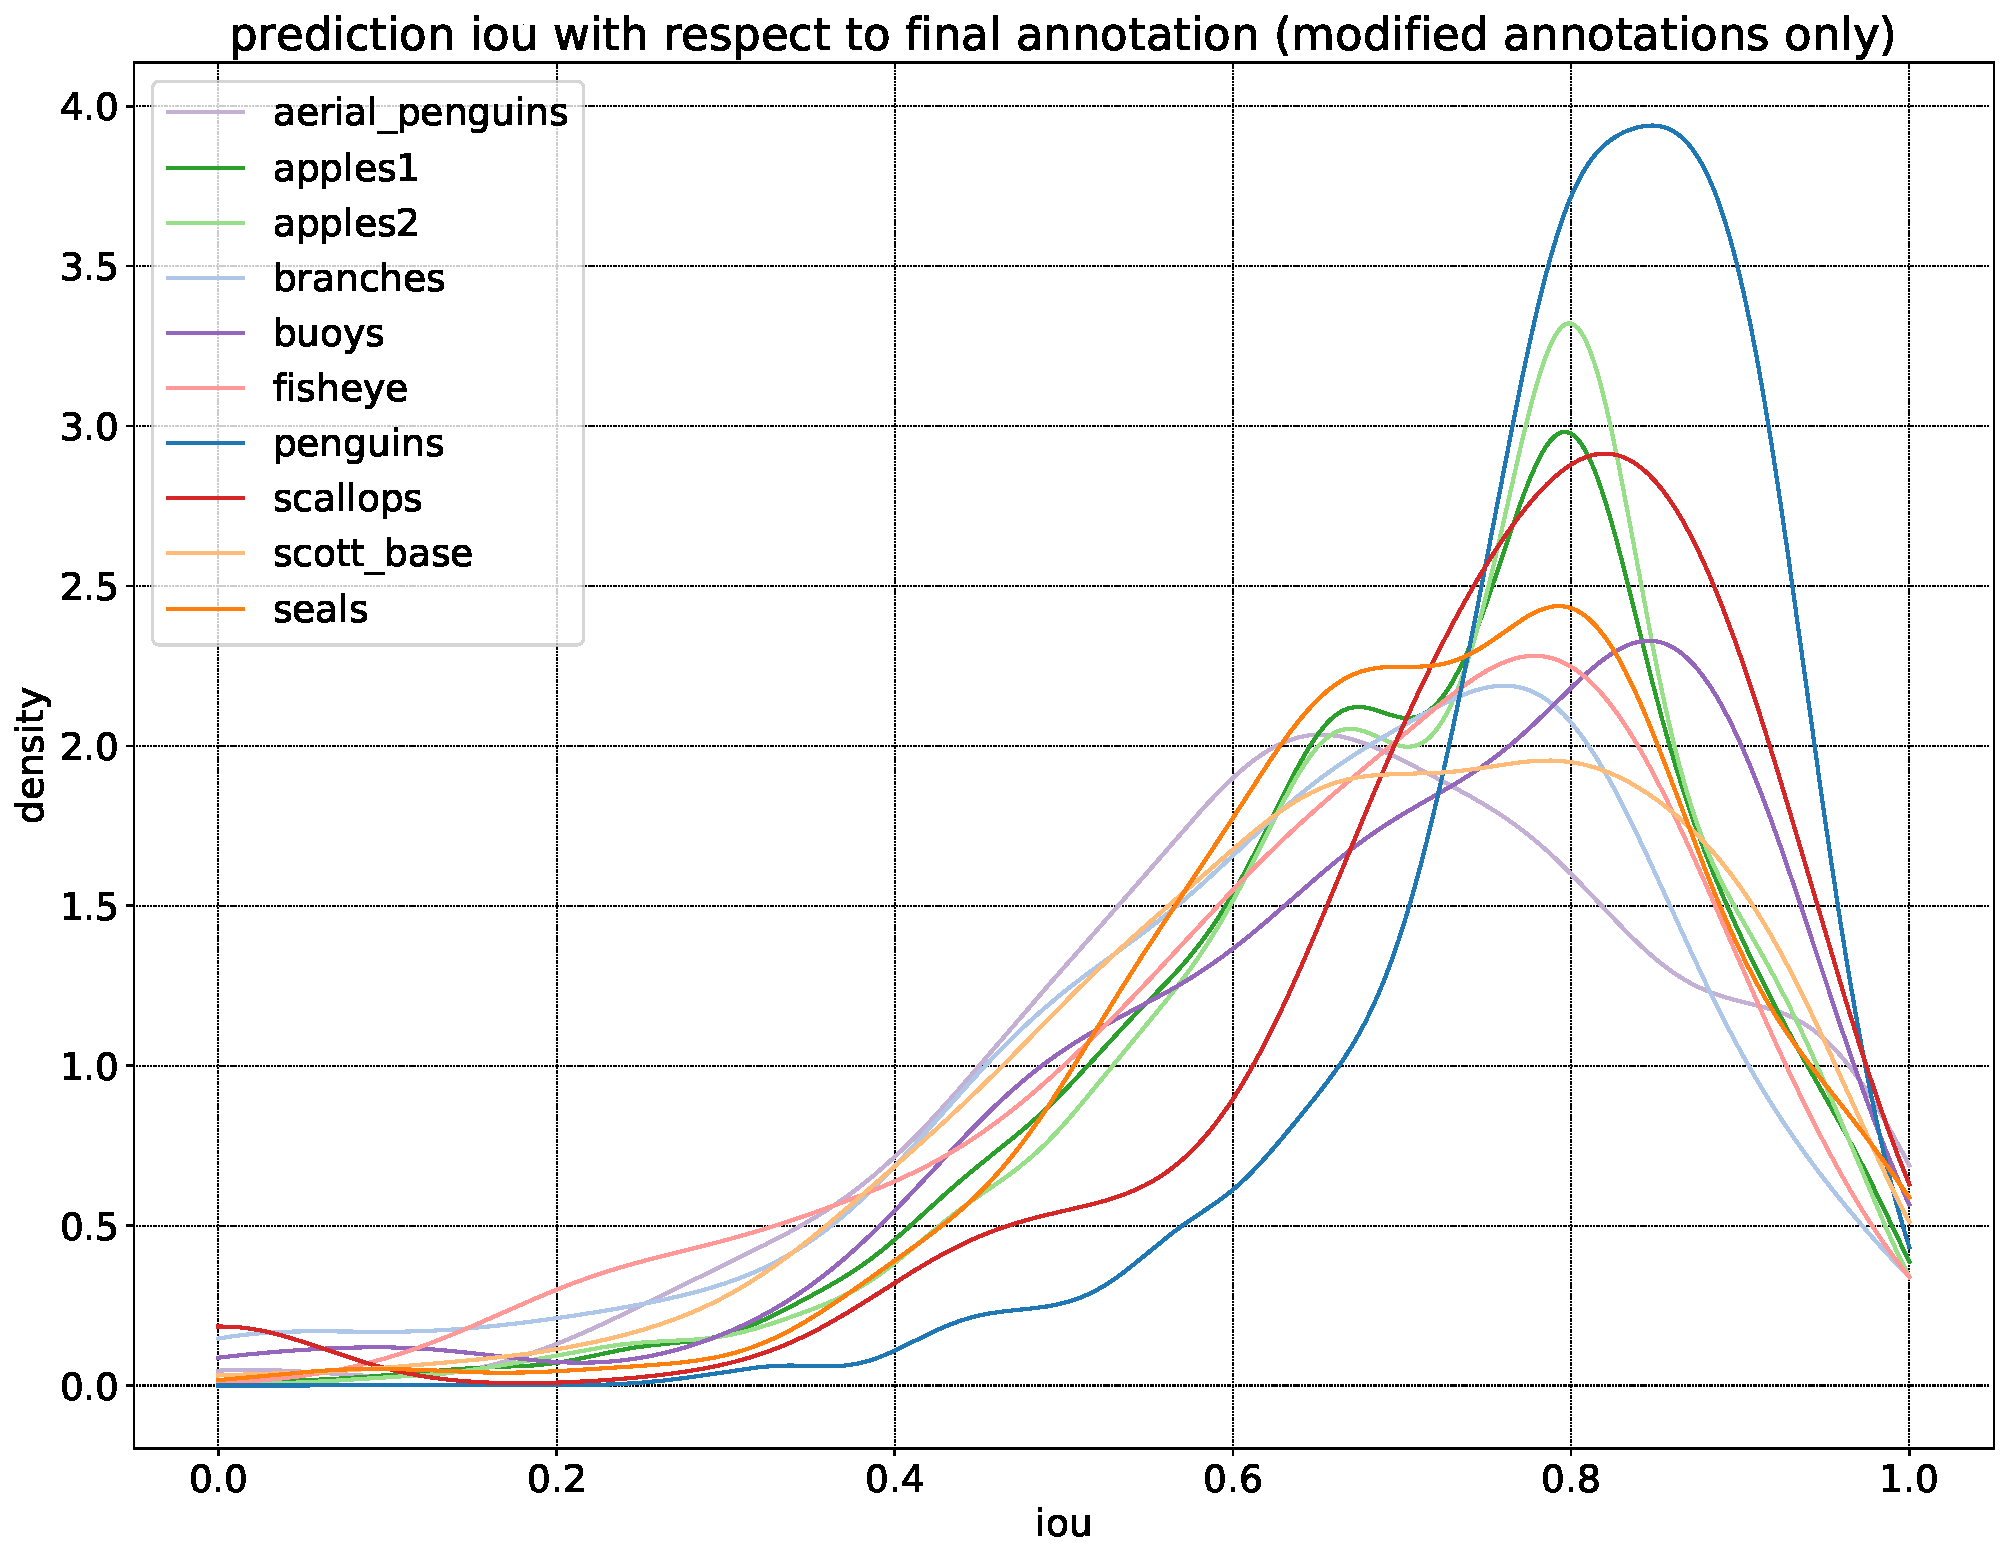
\includegraphics[width=1.0\linewidth]{charts/scatters/iou_dataset.pdf}
\caption{ Density plot of IoU for transformed annotations for each dataset }
\label{fig:density_iou}
\end{figure}



In order to verify any annotation (regardless if it was created by human annotation or machine detection), there exists an implicit localisation threshold. This threshold and the amount of variability can't be measured directly without an absolute ground truth, or by repeated annotation of the same images. It is possible however to analyse the magnitude of the corrections applied.

Human annotation has a certain amount of variability, from person to person and even annotations from the same person. For a large annotation effort a plan for annotation and quality controls can improve consistency



\subsection{Localisation vs. confidence}
\label{sec:localisation_confidence}

\begin{figure}[ht]
\centering
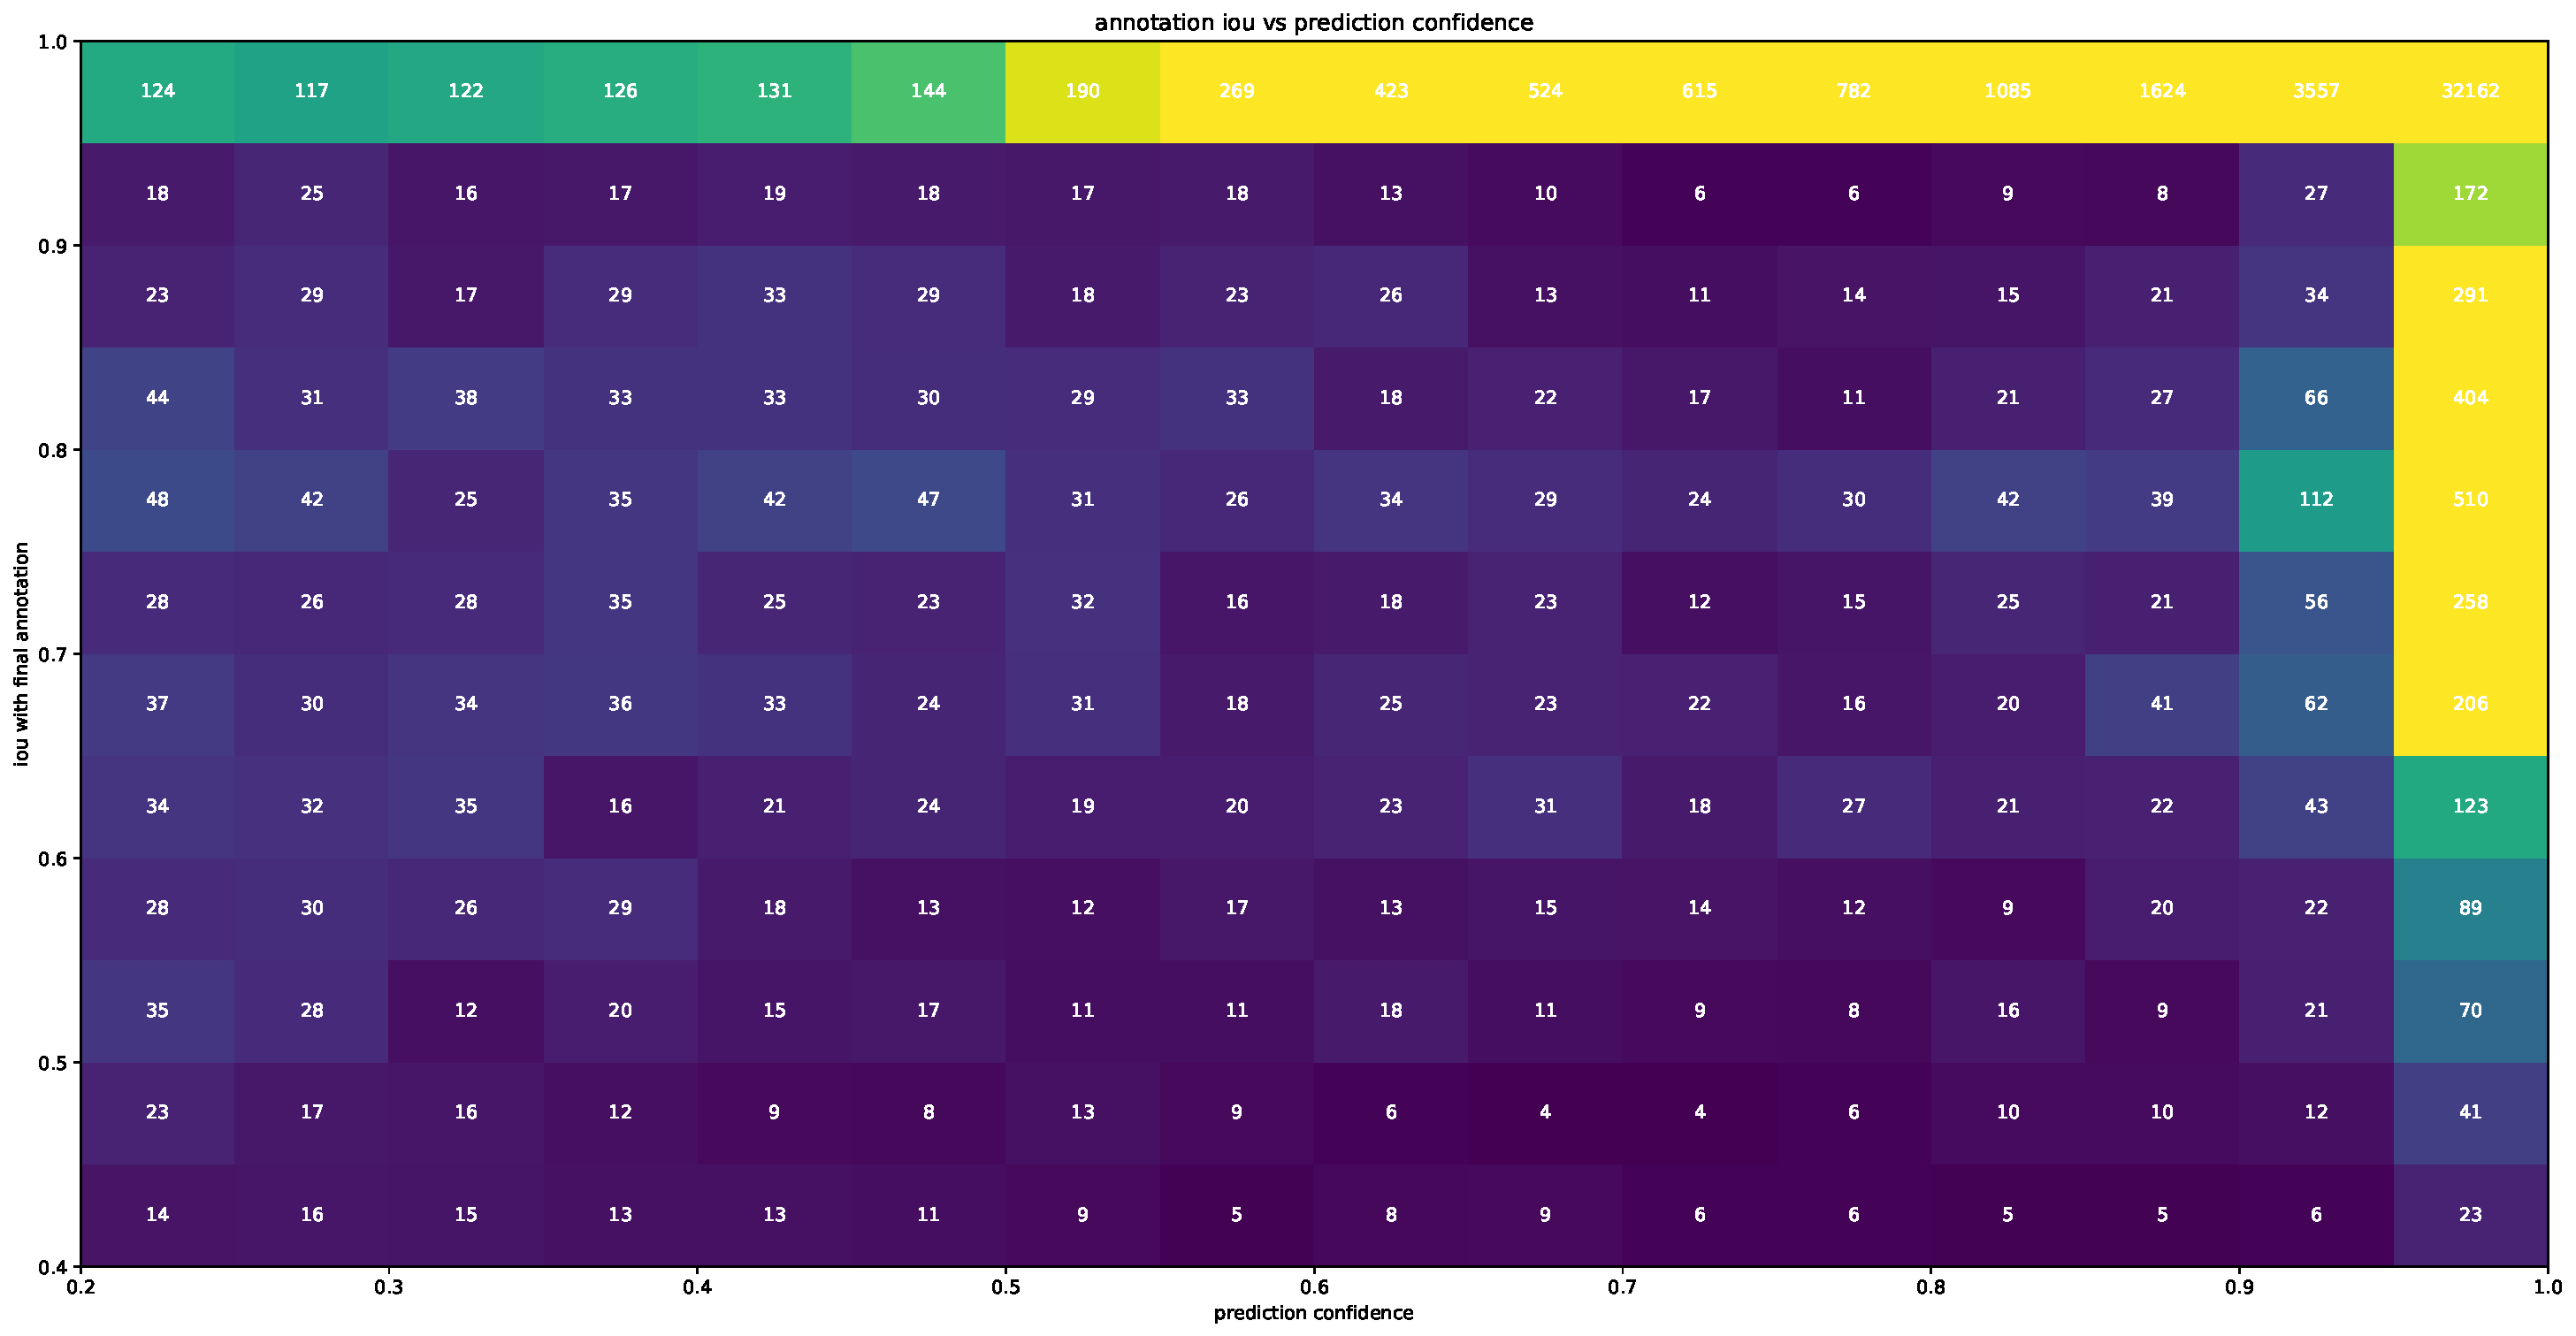
\includegraphics[width=1.0\linewidth]{charts/scatters/confidence_iou.pdf}
\caption{ IoU of detection with respect to final annotation vs. confidence, for detections (modified or otherwise) included as an annotation }
\label{fig:iou_confidence}
\end{figure}

One of the premises of providing the ability to pick and chose low confidence detections (using the two threshold method) is that weakly detected objects are often be localised well. Figure~\ref{fig:iou_confidence} shows that is the case, both a significant proportion final annotations had low confidence and  precise localisation (as well as a proportion having high confidence and imprecise localisation).


\begin{table}[h]
\caption{Breakdown by dataset of detections included as an annotation; confident if $ p > 0.7 $, precise if $ IoU > 0.85 $ with respect to final annotation} 
\noindent\resizebox{1.0\textwidth}{!}{%    
\begin{tabular}{l l l l l l l l || l}
& seals  & $seals_b$ & $apples^1$ & $apples^2$ & penguins & fisheye & branches & total  \\
\toprule
high confidence, imprecise & 1.2\%  & 0.4\%     & 5.1\%      & 7.9\%      & 7.5\%    & 1.4\%   & 5.3\%    & 5.5\%  \\
low confidence, precise & 7.2\%  & 6.3\%     & 6.5\%      & 5.5\%      & 1.2\%    & 5.6\%   & 7.5\%    & 5.5\%  \\
high confidence, precise   & 90.2\% & 93.1\%    & 81.5\%     & 80.0\%     & 89.7\%   & 89.9\%  & 79.6\%   & 83.7\% \\
\bottomrule
\end{tabular}
}
\end{table}

In the implementation of object detection neural networks such as the one used in this work (see chapter~\ref{chap:object_detection}) the sub-network for classification is separate from localisation and localisation is predicted for all anchor boxes regardless of classification performance. It is not surprising therefore that sometimes localisation is predicted well an yet the object is not classified well.




\subsection{ Apples comparison }
\label{sec:apples_comparison}


\begin{figure}[ht]
\centering
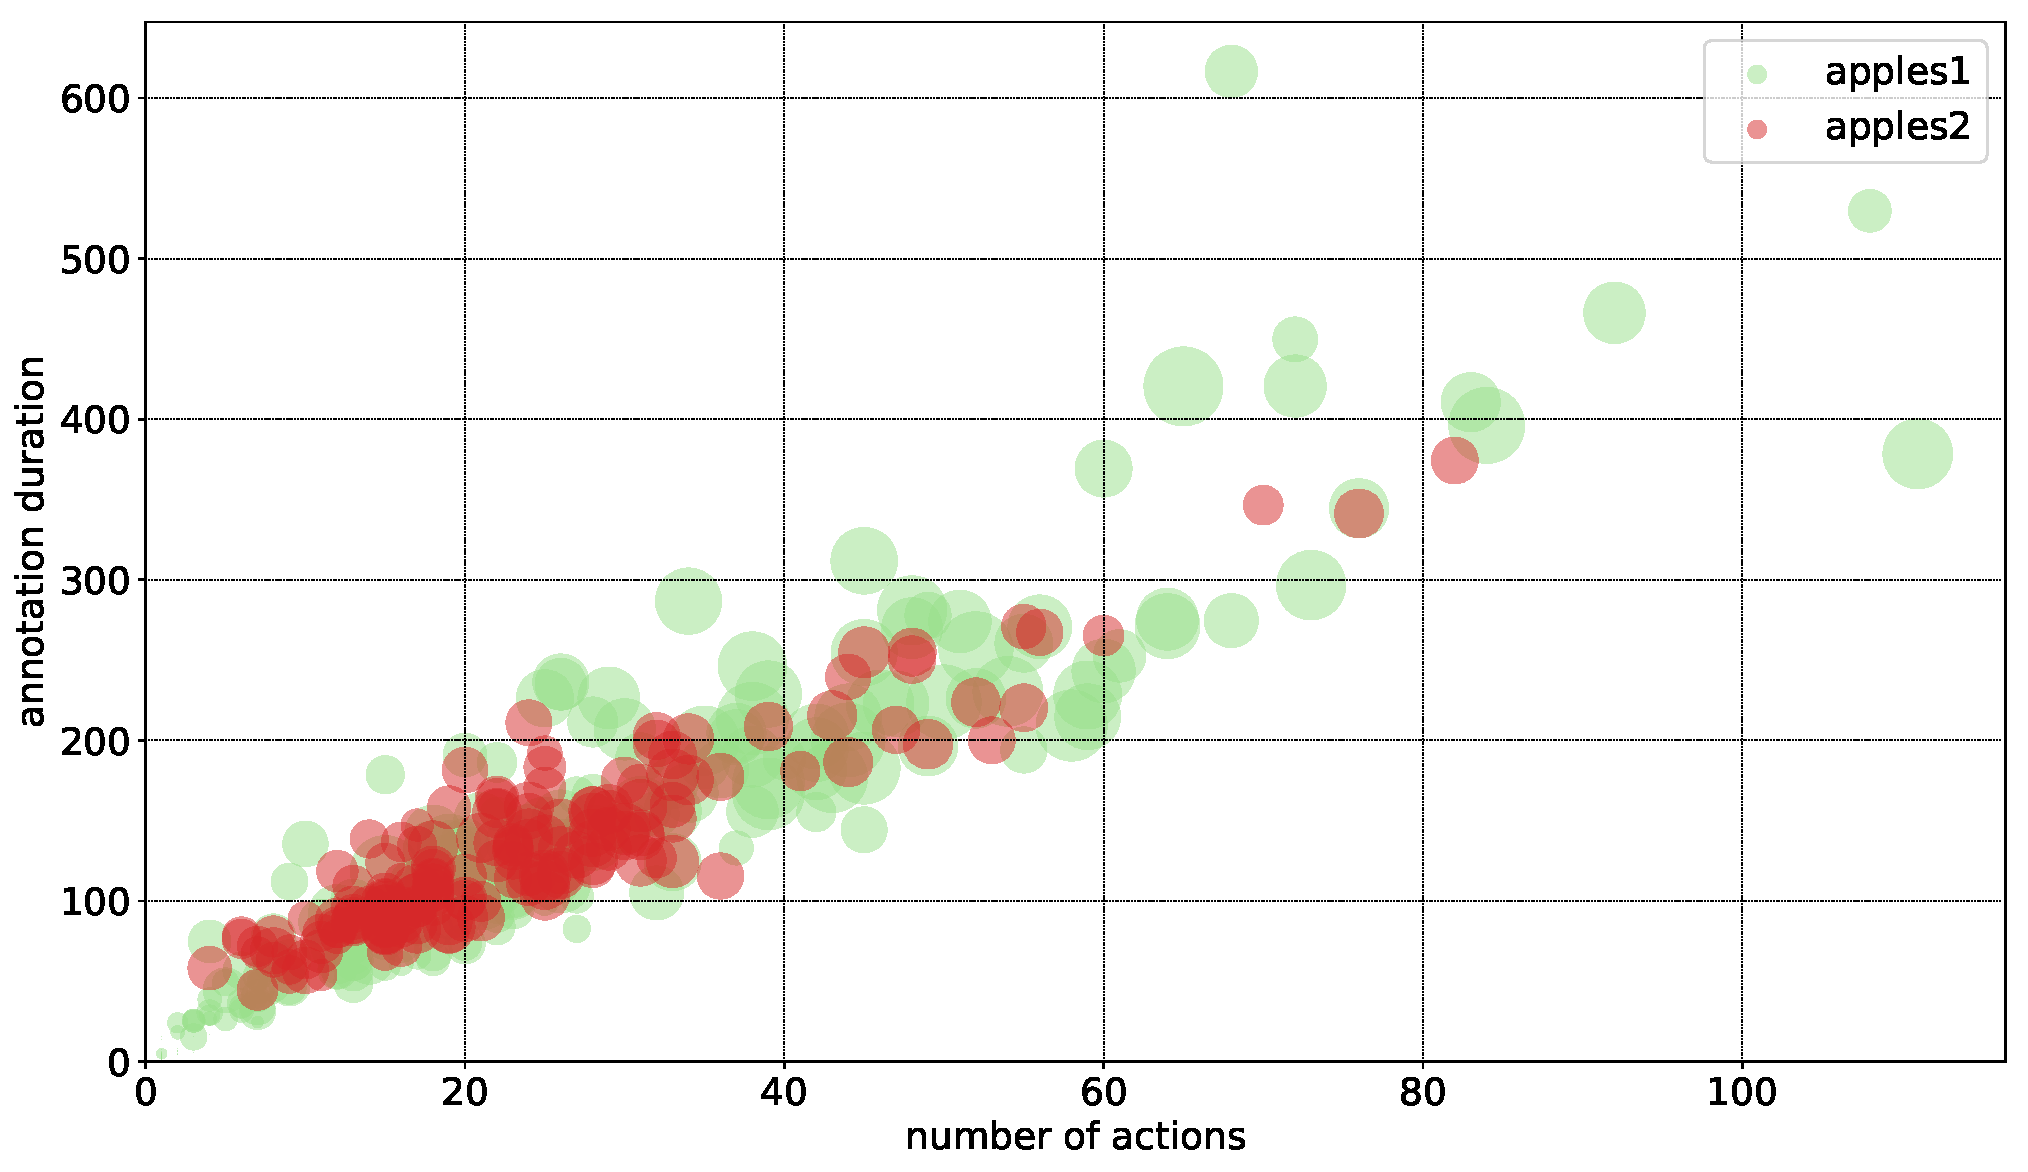
\includegraphics[width=1.0\linewidth]{charts/scatters/apples_scatter.pdf}
\caption{ Number of actions vs. annotation time, the area of the points represent number of instances }
\label{fig:apples_actions_time}
\end{figure}



\section{Case study: counting Adélie penguins from aerial photographs}
\label{sec:case_penguins}

\begin{figure*}[H]
\centering
\begin{subfigure}[t]{1.0\linewidth}
  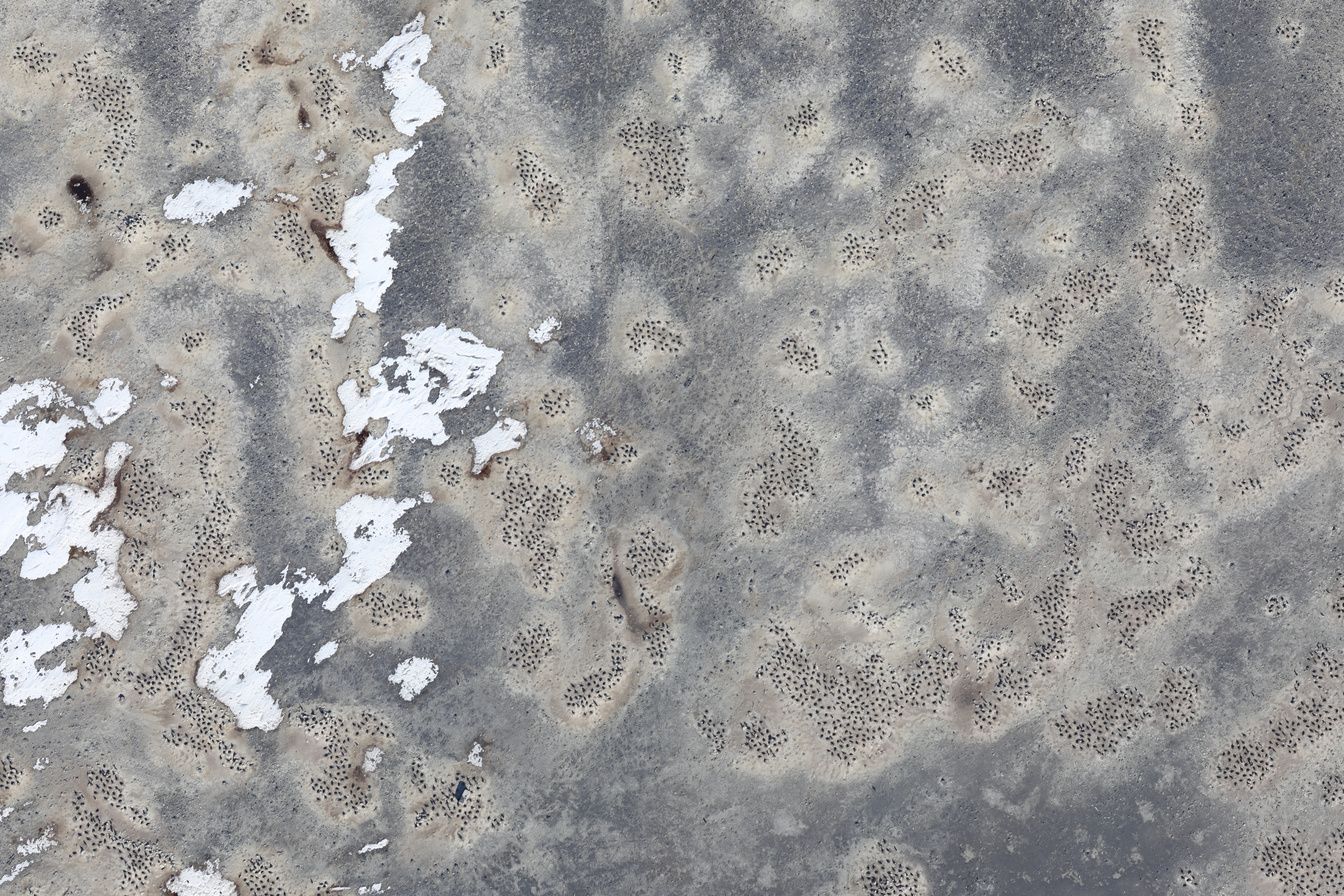
\includegraphics[width=0.475\linewidth]{figures/annotation/penguin/hallet_large.jpg}
  \hfill
  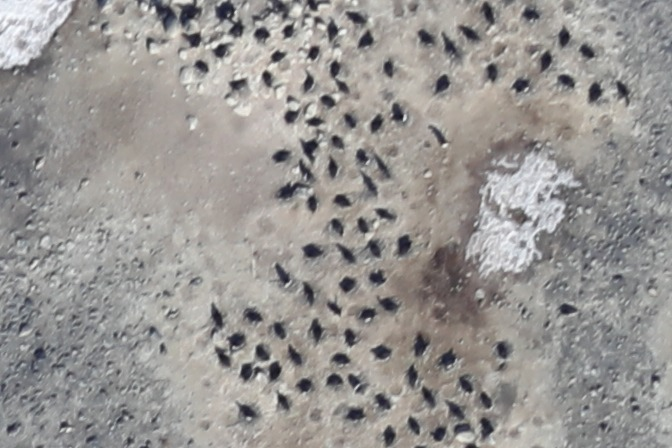
\includegraphics[width=0.475\linewidth]{figures/annotation/penguin/hallet.jpg}
  \caption{Cape Hallett 2017}
\end{subfigure}
\begin{subfigure}[t]{1.0\linewidth}
  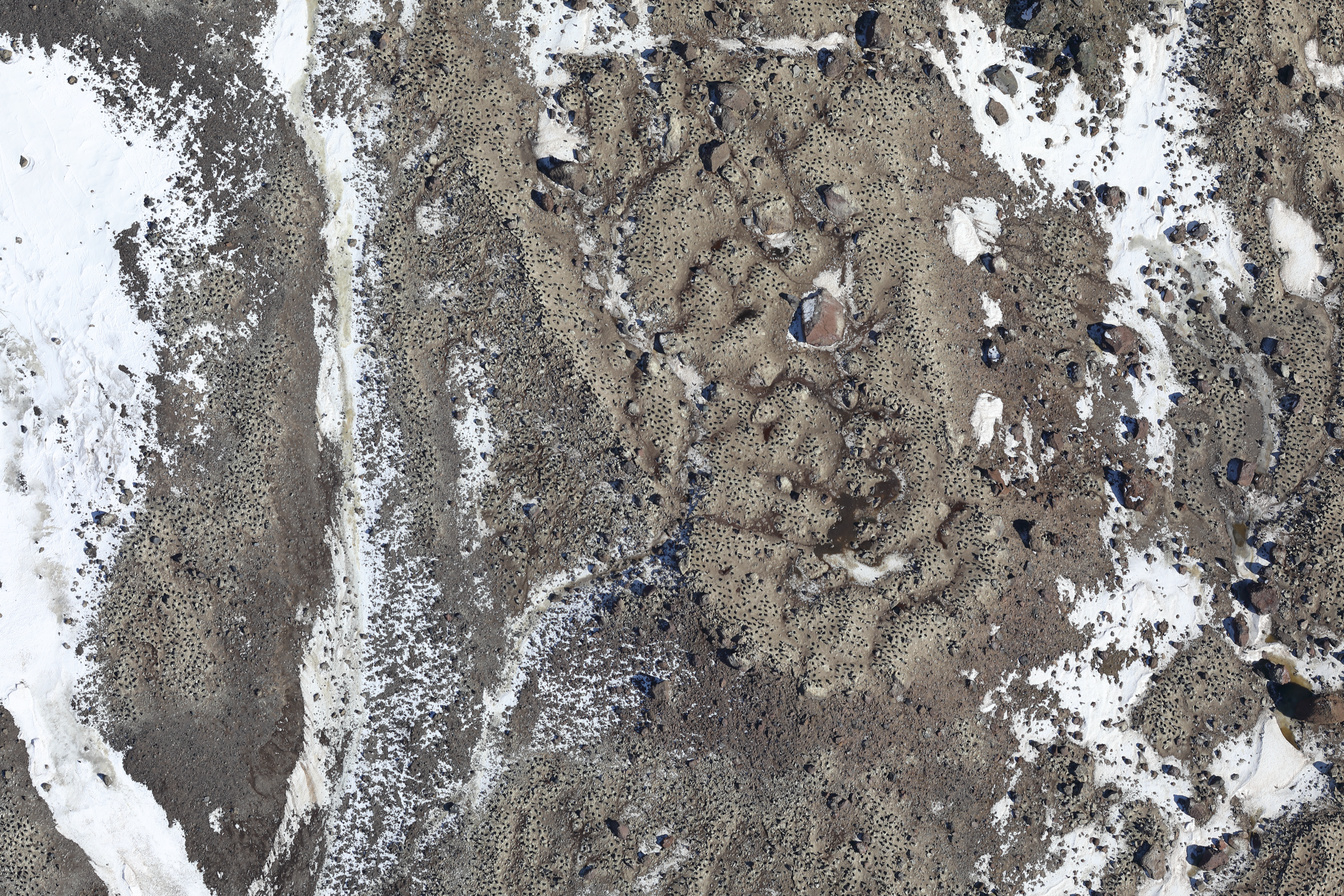
\includegraphics[width=0.475\linewidth]{figures/annotation/penguin/cotter_large.jpg}
  \hfill 
  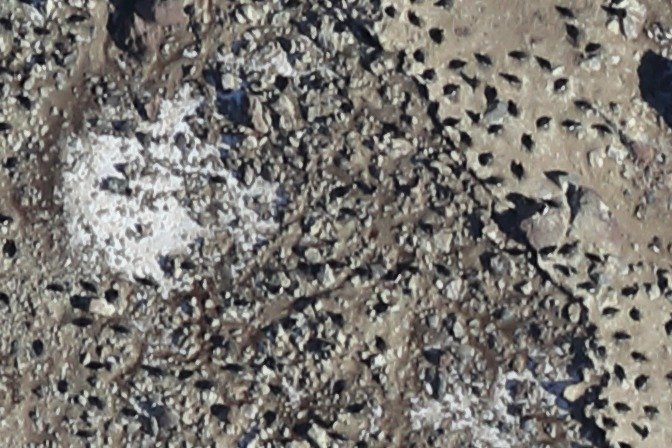
\includegraphics[width=0.475\linewidth]{figures/annotation/penguin/cotter.jpg}
  \caption{Cape Cotter 2017}
\end{subfigure}
\begin{subfigure}[t]{1.0\linewidth}
  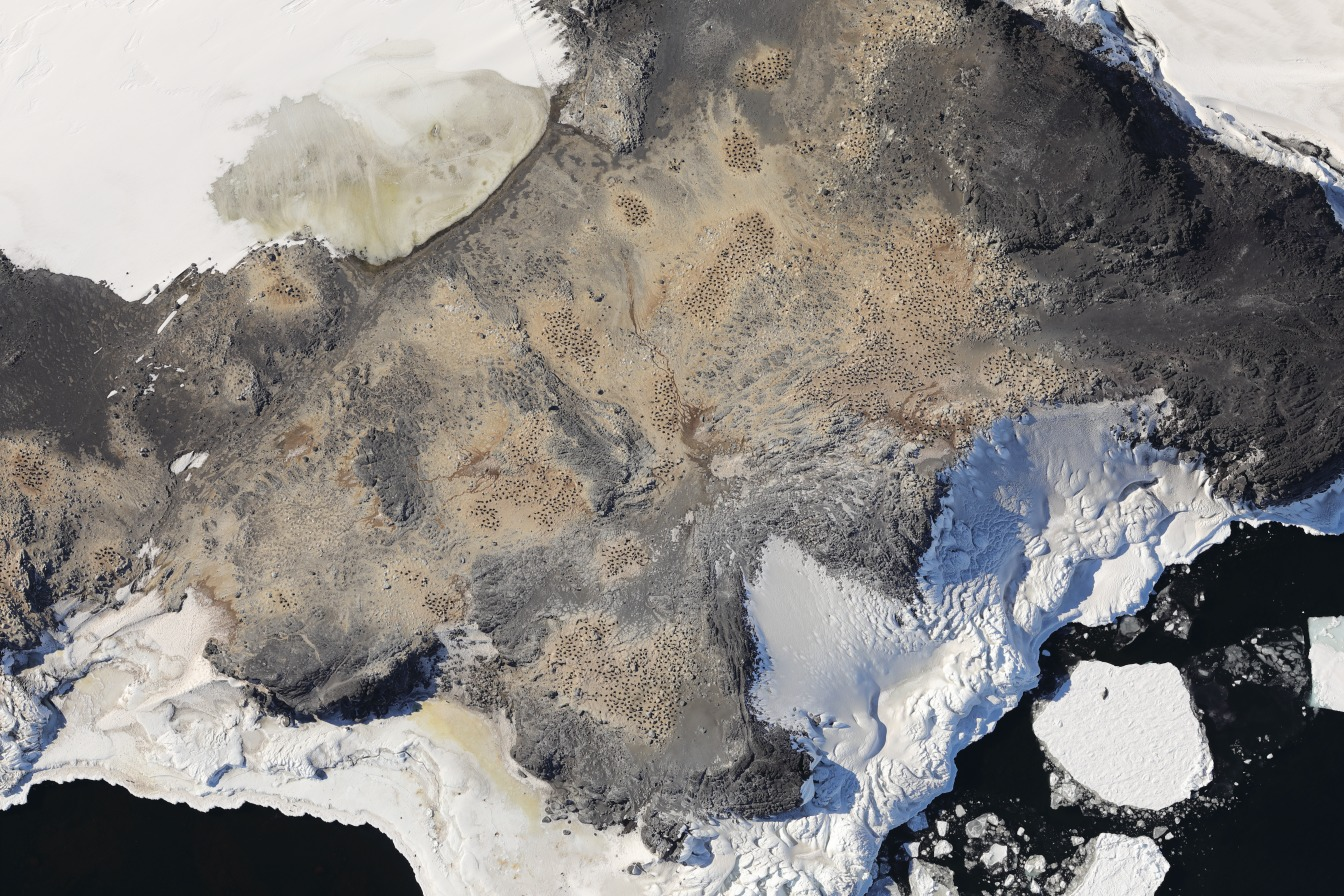
\includegraphics[width=0.475\linewidth]{figures/annotation/penguin/royds_large.jpg}
  \hfill
  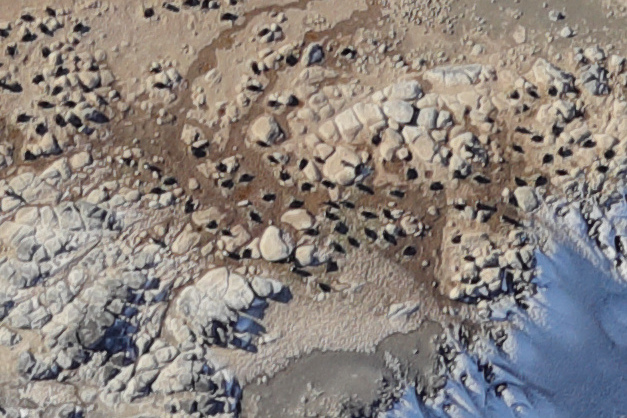
\includegraphics[width=0.475\linewidth]{figures/annotation/penguin/royds.jpg}
  \caption{Cape Royds 2017}
\end{subfigure}

\caption{Examples from the Adelie penguin census data taken in 2017. On the left hand column are images showing the zoomed out landscape, on the right are representative crops zoomed in.  In (a) an image from Cape Hallet image showing clearly visible, easy to identify penguins as dark patches. In (b) Cape Cotter showing many more difficult to identify penguins, often with a high degree of ambiguity not only for the machine learning algorithm but for a human annotator, in rocky areas especially shadows from rocks are very difficult to discern from penguins. In (c) Cape Royds, a smaller colony to the other two (and complete). In terms of ambiguity and uncertainty somewhere in-between. }
\label {fig:penguin_examples}
\end{figure*}


One potentially useful for verification based annotation is counting things, it provides some of the time savings of automatic inference but also the accuracy of human annotation because the machine predictions are all verified, and can begin without possessing an existing dataset or developing specific recognition methods. 

One of the sources of inspiration for this work in verification based annotation came from \cite{McNeill2011}, where a tool was created to semi-automatically count Adélie penguins from aerial photographs. The penguins are first automatically detected, then follows a verification process allowing a human annotator to mark false positives and false negatives. Their method for detecting penguins is to first detect penguin colonies which can often be done by the unique colour of the penguin guano. Individual penguins were then identified by thresholding and local minima detection and culling of long thin objects. 

The images (two of which can be seen in figure~\ref{fig:penguin_examples}), originate from aerial photographic surveys \cite{Lyver2014}, from high resolution photographs, taken from 2000-2500 feet. In the case of the two images from Cape Cotter and Hallet in figure~\ref{fig:penguin_examples}, the images are cropped from images of size $ 6720\times4480 $. The Cape Royds images are spliced together from three images with various areas masked out, this was done by filling in the overlapping and irrelevant areas using a paint program.

The study which has been conducted from 1981 until present, prior to 2010 involved manually counting individual penguins using a pin to manually mark penguins and avoid duplication. 


\subsection {Effect of image ambiguity}

One aspect which can be studied from the penguin survey images is how image based (aleatoric) uncertainty impacts the annotation process. It can be seen in figure~\ref{fig:penguin_examples} that between the three images from different geographical locations each has a different level of 

When significant ambiguity is present in the source images (aleatoric uncertainty), a challenge is presented not only for the object detector, but for the human annotator. Many of the penguin instances to the untrained eye appear very similar to the shadow cast by rocks and difficult to discern. The nature of the imagery from the different sites shown in figure~\ref{fig:penguin_examples} provide a test case to compare the effectiveness of verification with different levels of uncertainty in the source image. 

\subsection {Method}

Separately the three sets of penguins using the annotation tool. Each set was annotated twice (by different annotators, the second being the author) for the purpose  of comparing human consistency in annotation.

I used circular annotations to speed up the annotation process. For counting (especially at the resolution of individual penguins) the precise bounding box seems unnecessary, and not needed to distinguish overlapping instances. 

The very large original images were split into images of size $ 672\times448 $ (Cape Royds images were of similar size, but not exactly the same because the source images were of different size, rather than one big image like the other two). Image crops of those image, sized $ 300\times300 $ were then used during training.

In the first case the annotation was impacted by a bug where the anchor centres were incorrect by a small amount causing small localisation errors. Over time (and iteration of annotation and prediction), this had the undesirable effect of causing the circle centres to wander. In the second case, annotated by the author, this bug was fixed. Despite this problem it also provides an opportunity to study the effect of providing noisy annotation localisation.


\begin{table}[]
  \centering
    \caption{Statistics from the thee penguin sources. }
\begin{tabular}{llllll}
dataset     & counted & total minutes & counts per minute & validation $AP_{50}$ & percent unmodified \\
\toprule
$hallett$   & 4164    & 28.8          & 145               & 98.70     & 86.5\%   \\
$hallett_c$ & 4249    & 65.2          & 65.1              & 99.35     & 91.5\%   \\
$royds$     & 2783    & 30.7          & 90.6              & 88.73     & 88.1\%   \\
$royds_c$   & 2536    & 146           & 17.4              & 65.63     & 69.4\%   \\
$cotter$    & 6263    & 60.6          & 103               & 92.34     & 92.1\%   \\
$cotter_c$  & 6196    & 245           & 25.2              & 78.68     & 85.9\%  \\
\bottomrule
\end{tabular}
\end{table}





\subsection{Results and discussion}
 
The difference in difficulty can clearly be seen in the difference of mAP in figure~\ref{fig:penguin_statistics}, where the Cape Hallet penguins were detected with almost perfect accuracy, whereas Cape Royds was more difficult and Cape Cotter considerably more difficult. 

\subsection{ Localisation precision }
\label{sec:localisation_precision}

\begin{figure}[ht]
\centering
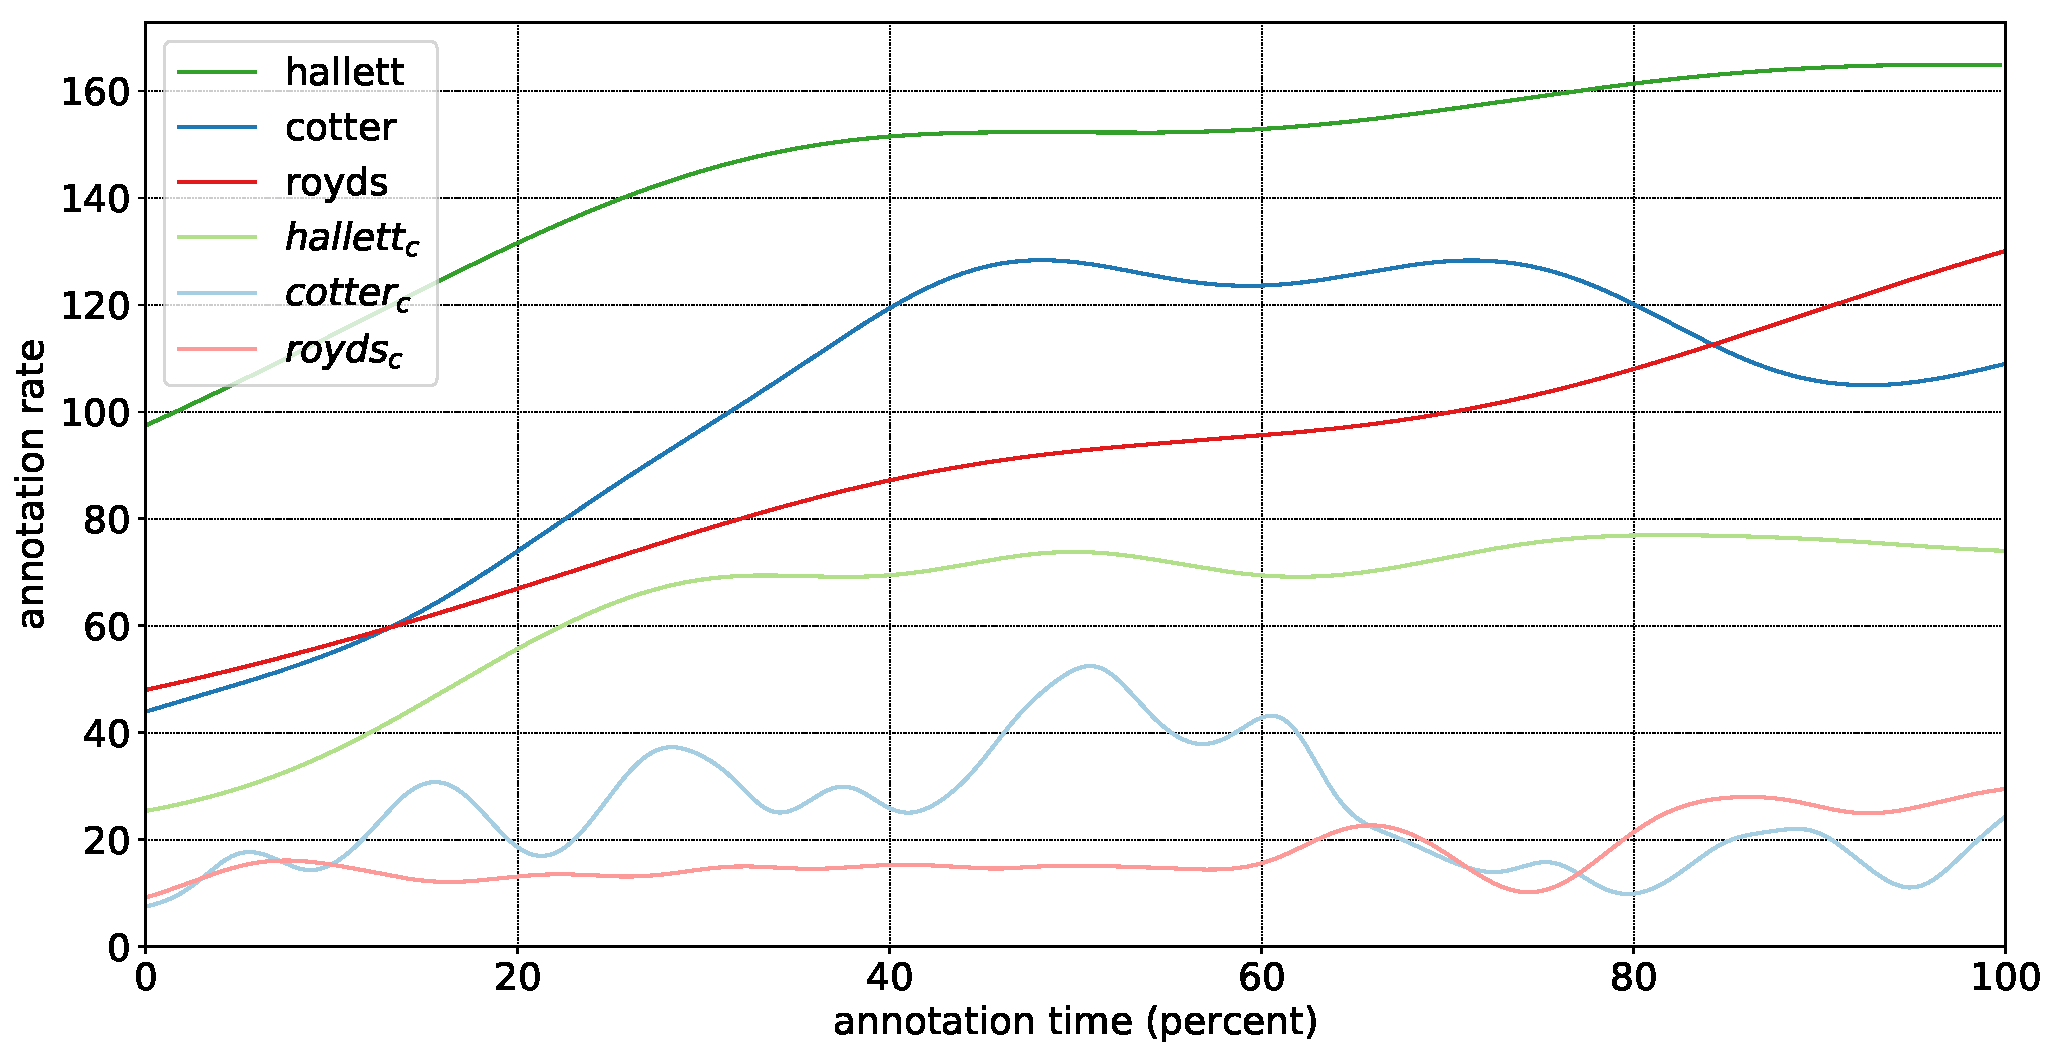
\includegraphics[width=1.0\linewidth]{charts/aerial_penguins/summaries/instance_rates.pdf}
\caption{ Rates of counting for the different image subsets }
\label{fig:penguin_rates}
\end{figure}



\begin{figure}[ht]
\centering
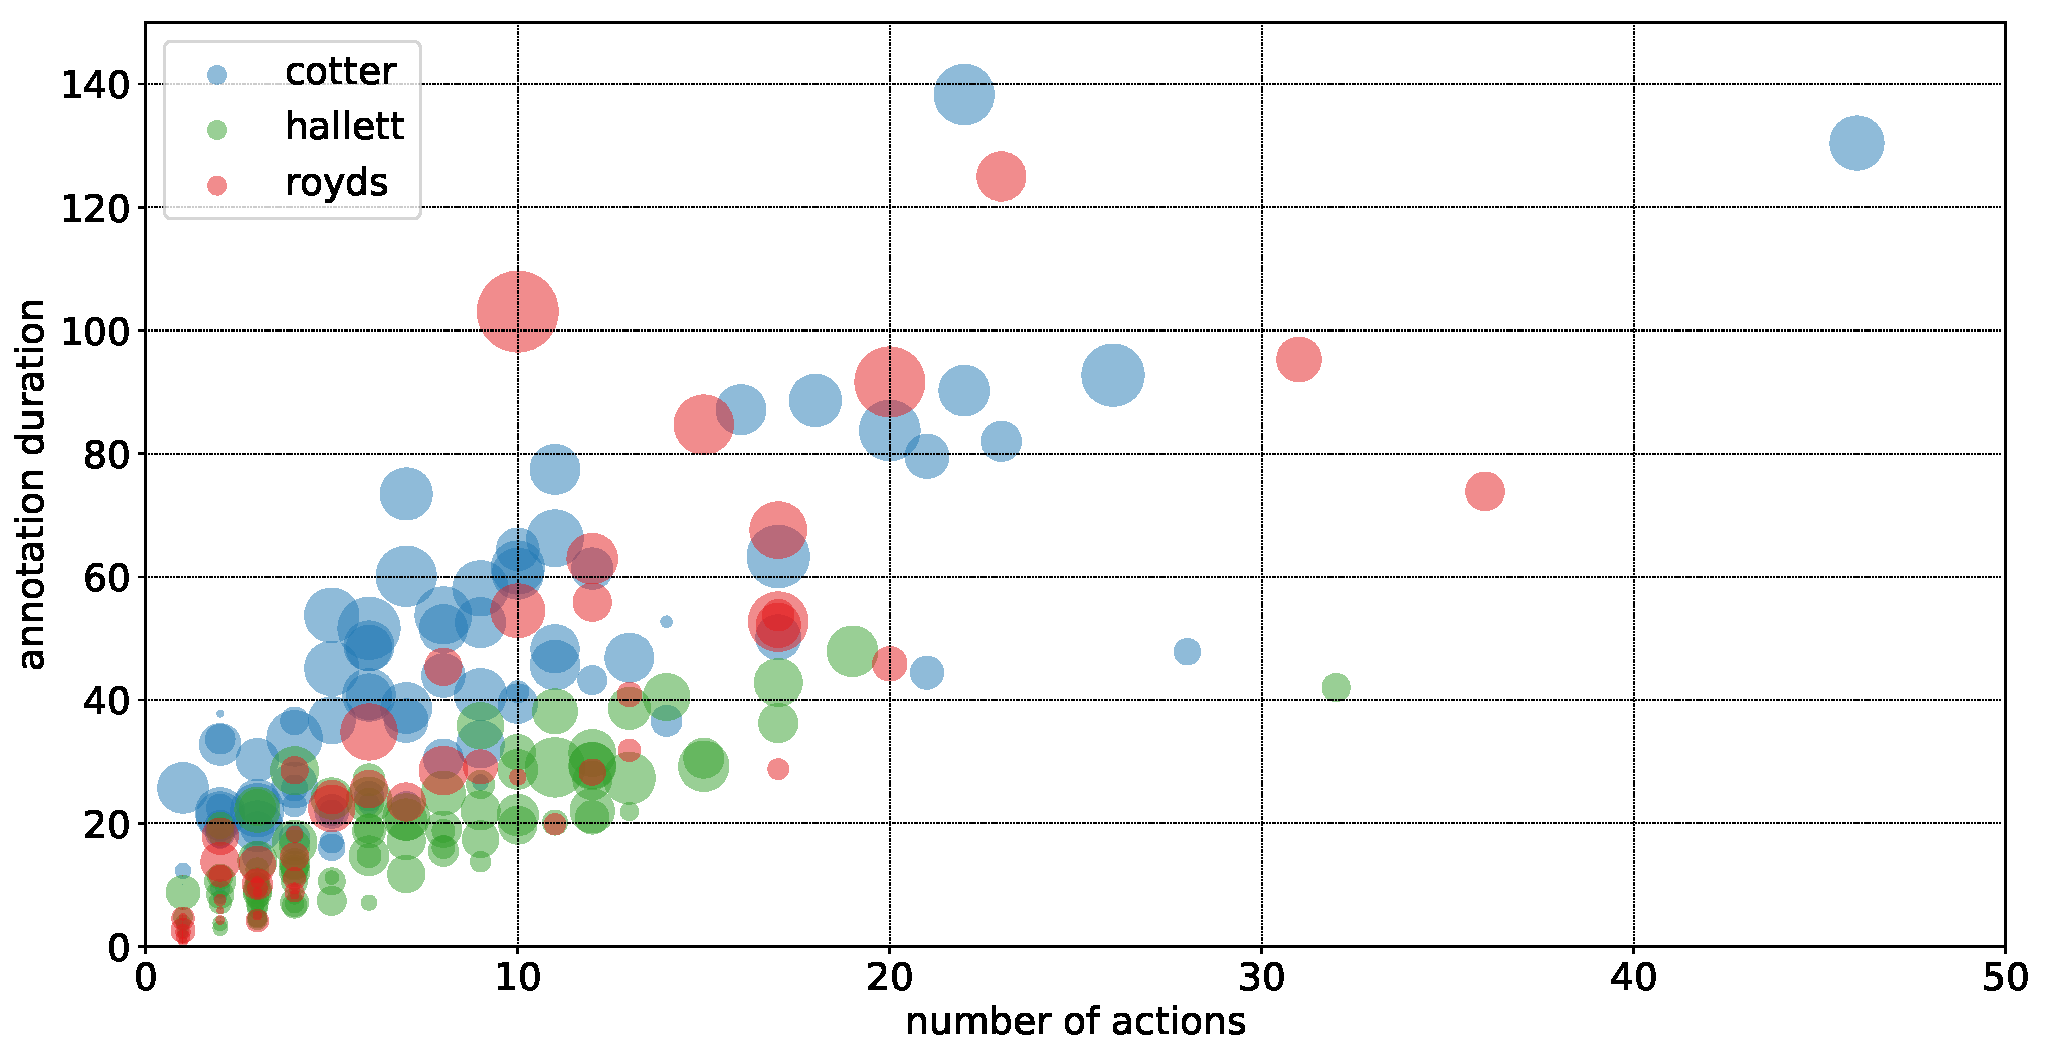
\includegraphics[width=1.0\linewidth]{charts/aerial_penguins/actions_time_a.pdf}
\caption{ Number of actions vs. counting duration for each image between image subsets, the area of each point is proportional to the number of instances counted }
\label{fig:actions_time_penguins}
\end{figure}


\subsection{Case Study: Analysing Waddell Seal Counts}
\label{sec:case_seals}


\begin{figure*}[h!]
\centering
\begin{subfigure}[t]{1.0\linewidth}
  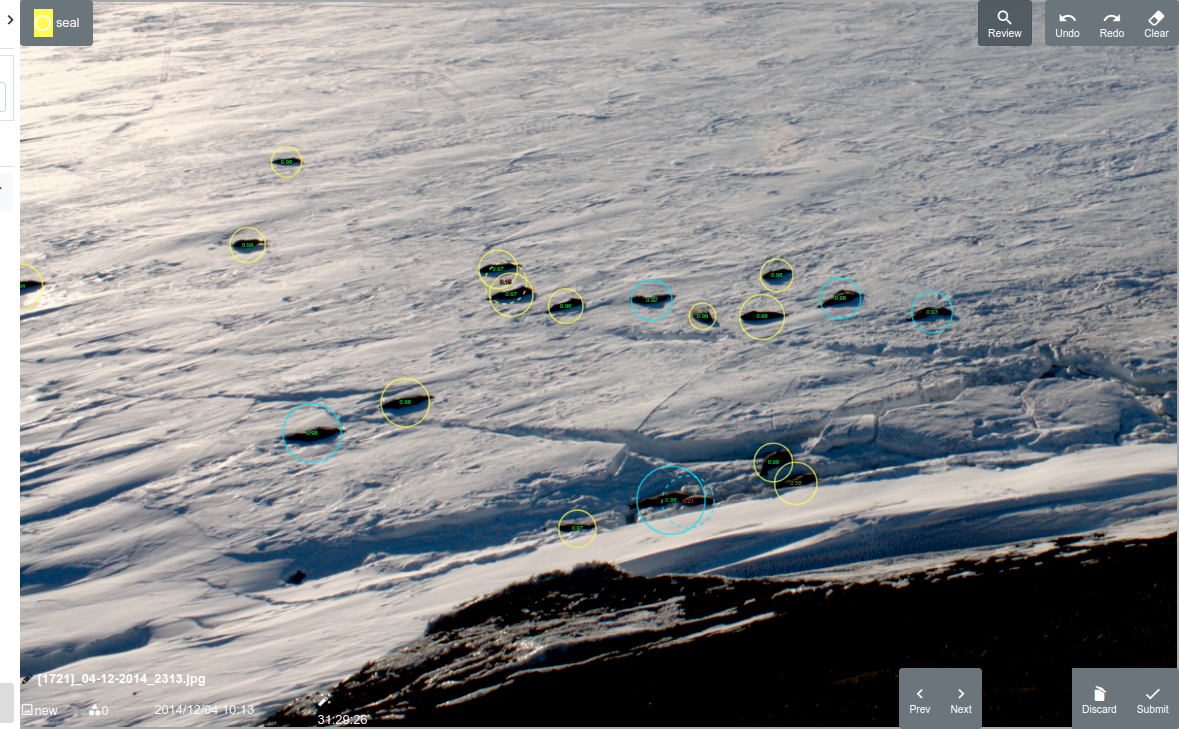
\includegraphics[width=0.475\linewidth]{figures/annotation/screenshots/seals_small2.png}
  \hfill
  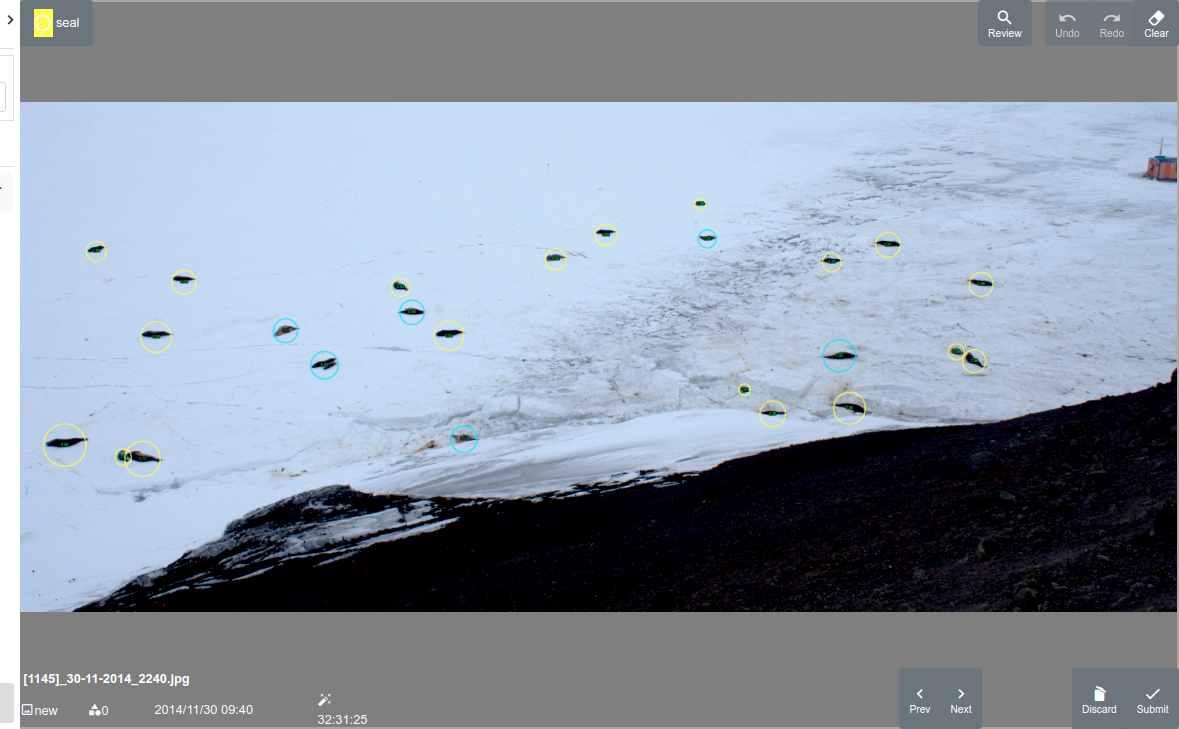
\includegraphics[width=0.475\linewidth]{figures/annotation/screenshots/seals_small.png}
  \caption{}
\end{subfigure}

\begin{subfigure}[t]{1.0\linewidth}
  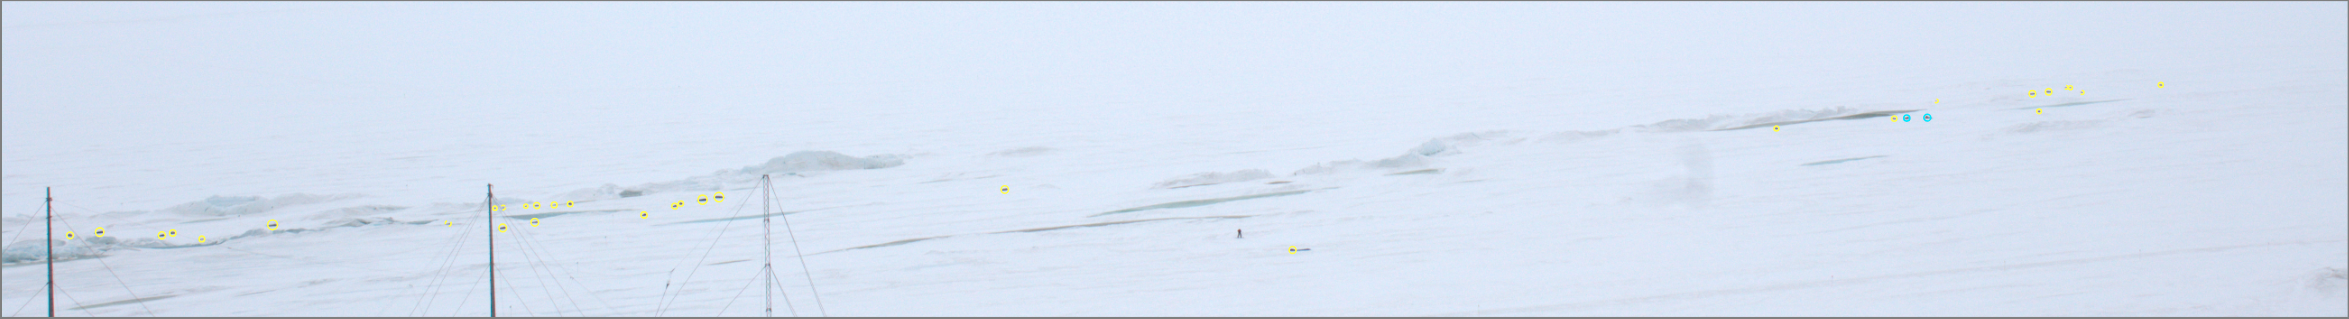
\includegraphics[width=1.0\linewidth]{figures/annotation/screenshots/cam_c.png}
\end{subfigure}

\begin{subfigure}[t]{1.0\linewidth}
  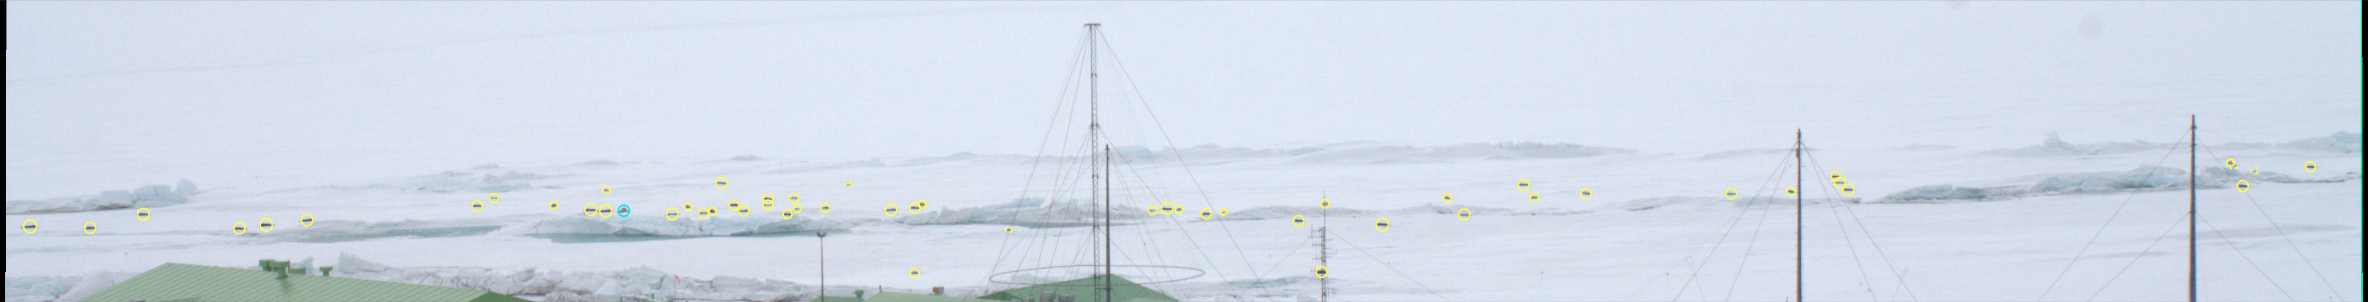
\includegraphics[width=1.0\linewidth]{figures/annotation/screenshots/cam_b.png}
  \caption{}
\end{subfigure}



\caption{ }
\label {fig:weddell_images}
\end{figure*}



\section{Discussion}


\subsection{Number of instances}
\label{sec:instances_discussion}

The instance distribution in each image has clear implications for verification based image annotation. Verifying several instances at once can be more efficient than one at a time, but verifying too many instances concurrently increases cognitive load (the very problem human in the loop machine learning seeks to address). 

Despite the ability to zoom into a small part of an image, in order to submit an image the user must review the whole image or remember which parts have been checked. For this reason when images become excessively large they should be split into pieces which can be easily verified without too much use of navigation.

This can be similar to a user interface for navigating search results, showing several results at once is much faster for a user to peruse than showing them one by one. However, if too many results are shown on each page results become lost in the crowd. A pair of studies found users do not look at results beyond 30 per page \cite{PunchoojitLumpapun2017, Zhou2007}.

The dual threshold approach helped in this regard by highlighting areas of uncertainty. For some datasets \emph{penguin surveys} and \emph{apples1}, \emph{apples2} the number of instances made it hard to keep track of progress when verifying the whole image. Combined with uncertain instances which are difficult to see without zooming, checking to ensure all annotations are present becomes difficult.

The dataset \emph{scott base} also suffers a little from this problem. The images are much wider than they are long, making navigation somewhat tedious and verifying the whole image much harder by having to zoom right out to check the whole image.

In future some method of marking parts of image as checked may help here.


